\documentclass[ruledheader,noindentfirst,anapcustomindent,abntfigtabnum,tocpage=plain]{def_and_cls/abnt}
\usepackage{amsmath, amssymb, amsthm, verbatim, amsfonts, amstext}
%\usepackage[latin1]{inputenc}
\usepackage[brazilian]{babel}
\usepackage[utf8]{inputenc}
\usepackage[T1]{fontenc}
\usepackage{styles/dropping}
\usepackage{graphicx}
\usepackage[hang,small,bf]{caption}
\usepackage[abnt-etal-list=0,abnt-etal-text=it,abnt-and-type=&,abnt-emphasize=bf,abnt-full-initials=yes,alf,bibjustif]{styles/abntcite}
\usepackage{fancyhdr}
\usepackage{makeidx}
\usepackage[none]{hyphenat}
\usepackage{color}
\usepackage{subfig}
\usepackage{styles/algorithms}
\usepackage{algorithmic}
\usepackage{mdwlist}
\usepackage{bm}
\usepackage[titletoc,title]{appendix}
\usepackage{ltxtable}
\usepackage{longtable}
\usepackage{supertabular}
\usepackage{indentfirst}
\usepackage{color}
\usepackage{icomma}

% \usepackage{biblatex} %Imports biblatex package
% \addbibresource{mybibliography.bib} %Import the bibliography file

\usepackage[
    backend=biber,
    style=alphabetic,
    sorting=ynt
]{biblatex}

\addbibresource{bib.bib} %Imports bibliography file

\usepackage[table,xcdraw]{xcolor}
\usepackage{pdfpages}

\usepackage{adjustbox}
\usepackage{tabularray}
\usepackage{xurl}

\sloppy


%
%Tradução do pacote Algorithm para portugues
%
\renewcommand{\algorithmicrequire}{\textbf{Entrada:}}
\renewcommand{\algorithmicensure}{\textbf{Saída:}}
\renewcommand{\algorithmicend}{\textbf{fim}}
\renewcommand{\algorithmicif}{\textbf{se}}
\renewcommand{\algorithmicthen}{\textbf{então}}
\renewcommand{\algorithmicelse}{\textbf{senão}}
\renewcommand{\algorithmicelsif}{\algorithmicelse \, \algorithmicif}
\renewcommand{\algorithmicendif}{\algorithmicend \, \algorithmicif}
\renewcommand{\algorithmicfor}{\textbf{para}}
\renewcommand{\algorithmicforall}{\textbf{para todo}}
\renewcommand{\algorithmicdo}{\textbf{fazer}}
\renewcommand{\algorithmicendfor}{\algorithmicend \, \algorithmicfor}
\renewcommand{\algorithmicwhile}{\textbf{enquanto}}
\renewcommand{\algorithmicendwhile}{\algorithmicend \, \algorithmicwhile}
\renewcommand{\algorithmicloop}{\textbf{laço}}
\renewcommand{\algorithmicendloop}{\algorithmicend \, \algorithmicloop}
\renewcommand{\algorithmicrepeat}{\textbf{repetir}}
\renewcommand{\algorithmicuntil}{\textbf{até}}
\renewcommand{\algorithmiccomment}[1]{\{#1\}}
\renewcommand{\listalgorithmname}{Lista de Algoritmos}
\floatname{algorithm}{Algoritmo}
%%%%%%%%%%%%%%%%%%%%%%%%%%%%%%%%%%%%%%%%%%%%%%%%%%%%%%%%%%%%%%%%%%%%%%%%%%%%%%%%%%%

\makeindex

%%%% O arquivo modelosCAP.tex possui as definições para ciação do estilo de capítulo (fonte de título, barras horizontais, etc.)
% ele não gera texto de saída, é um arquivo de configuração somente
%
%Estilo de formatação de capítulos

\makeatletter
\newcommand{\thechapterwords}
{ \ifcase \thechapter\or 1\or 2\or 3\or 4\or 5\or6\or 7\or 8\or 9\or 10\or 11\fi}

\def\@makechapterhead#1{%
\vspace*{10\p@}%
{\parindent \z@  \reset@font

\scshape \@chapapp{} \thechapterwords
\quad %
\par\nobreak
\vspace*{10\p@}%
\interlinepenalty\@M
\hrule
\vspace*{10\p@}%
\Huge \bfseries #1\par\nobreak
\par
\vspace*{10\p@}%
\hrule
\vskip 40\p@
}}
\def\@makeschapterhead#1{%
\vspace*{10\p@}%
{\parindent \z@ \centering \reset@font
\par\nobreak
\vspace*{10\p@}%
\interlinepenalty\@M
\hrule
\vspace*{10\p@}%
\Huge \bfseries #1\par\nobreak
\par
\vspace*{10\p@}%
\hrule
\vskip 40\p@
%\vskip 100\p@
}}
%%%%%%%%%%%%%%%%%%%%%%%%%%%%%%%%%%%%%%%%%%%%%%%FIM DO PREAMBULO%%%%%%%%%%%%%%%%%%%%%%%%%%%%%%%%%%%%%%%%%%%%%%%%%%%%%%%%%%%%%%%%%%


\begin{document}

%%%%% IMPORTANTE: ALTERA O TEXTO ENTRE ARIAL E TIMES NEW ROMAN (ALTERNAR OS COMENTÁRIOS)
%
%%%%%%%%%%%%%%%%%%%%%PARA UTILIZAR ARIAL%%%%%%%%%%%%%%%%%%%%%%%
%
\fontfamily{phv}                    %fonte Arial
\renewcommand{\rmdefault}{phv}      %
%
%%%%%%%%%%%%%%%%%%%%%PARA UTILIZAR TIMES%%%%%%%%%%%%%%%%%%%%%%%
%
%\fontfamily{ptm}               %fonte Times
%\renewcommand{\rmdefault}{ptm} %
%
%%%%%%%%%%%%%%%%%%%%%%%%%%%%%%%%%%%%%%%%%%%%%%%%%%%%%%%%%%%%%%%

%%%%%%%%%%%%%Arquivos .tex com os elementos pré-textuais
%
\thispagestyle{empty}

\vfill
 \begin{center}
    {\large\bfseries ESCOLA POLITÉCNICA DA USP} \\
    \vspace*{1in}
    \begin{figure}[h]
     \centering
            
\includegraphics[width=10cm]{figures/Logo_Poli.jpg}\\
     \end{figure}
    \vspace*{1in}
    \large\bfseries Obtenção e análise de dados referentes à condução de carros
    
    \vspace{1.5cm}
    ANTONIO PINHEIRO DA SILVA JUNIOR - 9004355\\
    ARTHUR PIRES DA FONSECA - 10773096\\
    GABRIEL MORGHETT GABOARDI - 10773968\\
    \vfill
    \large\bfseries{ SÃO PAULO \\ 2023}
\end{center}

\normalsize
\begin{titlepage}
\vfill
\begin{center}
    \vspace{2cm}
    {\Large \textsc{Obtenção e análise de dados referentes à condução de carros}\\}
    \vspace{1cm}
    \hspace{.45\linewidth}
    \begin{minipage}{.50\linewidth}

            Trabalho apresentado à Escola Politécnica da Universidade de São Paulo para
            o Trabalho de Conclusão de Curso em Engenharia de Computação.
            São Paulo
            2020

            \vspace{0.5 cm}

            Orientador:     Prof. Dr. Edson Toshimi Midorikawa\\
            Co-orientador: Prof. Dr. Reginaldo Arakaki\\
    
    \end{minipage}

    \vspace{2cm}
    \vfill
    {\large SÃO PAULO\\ 2022}
\end{center}

\end{titlepage}
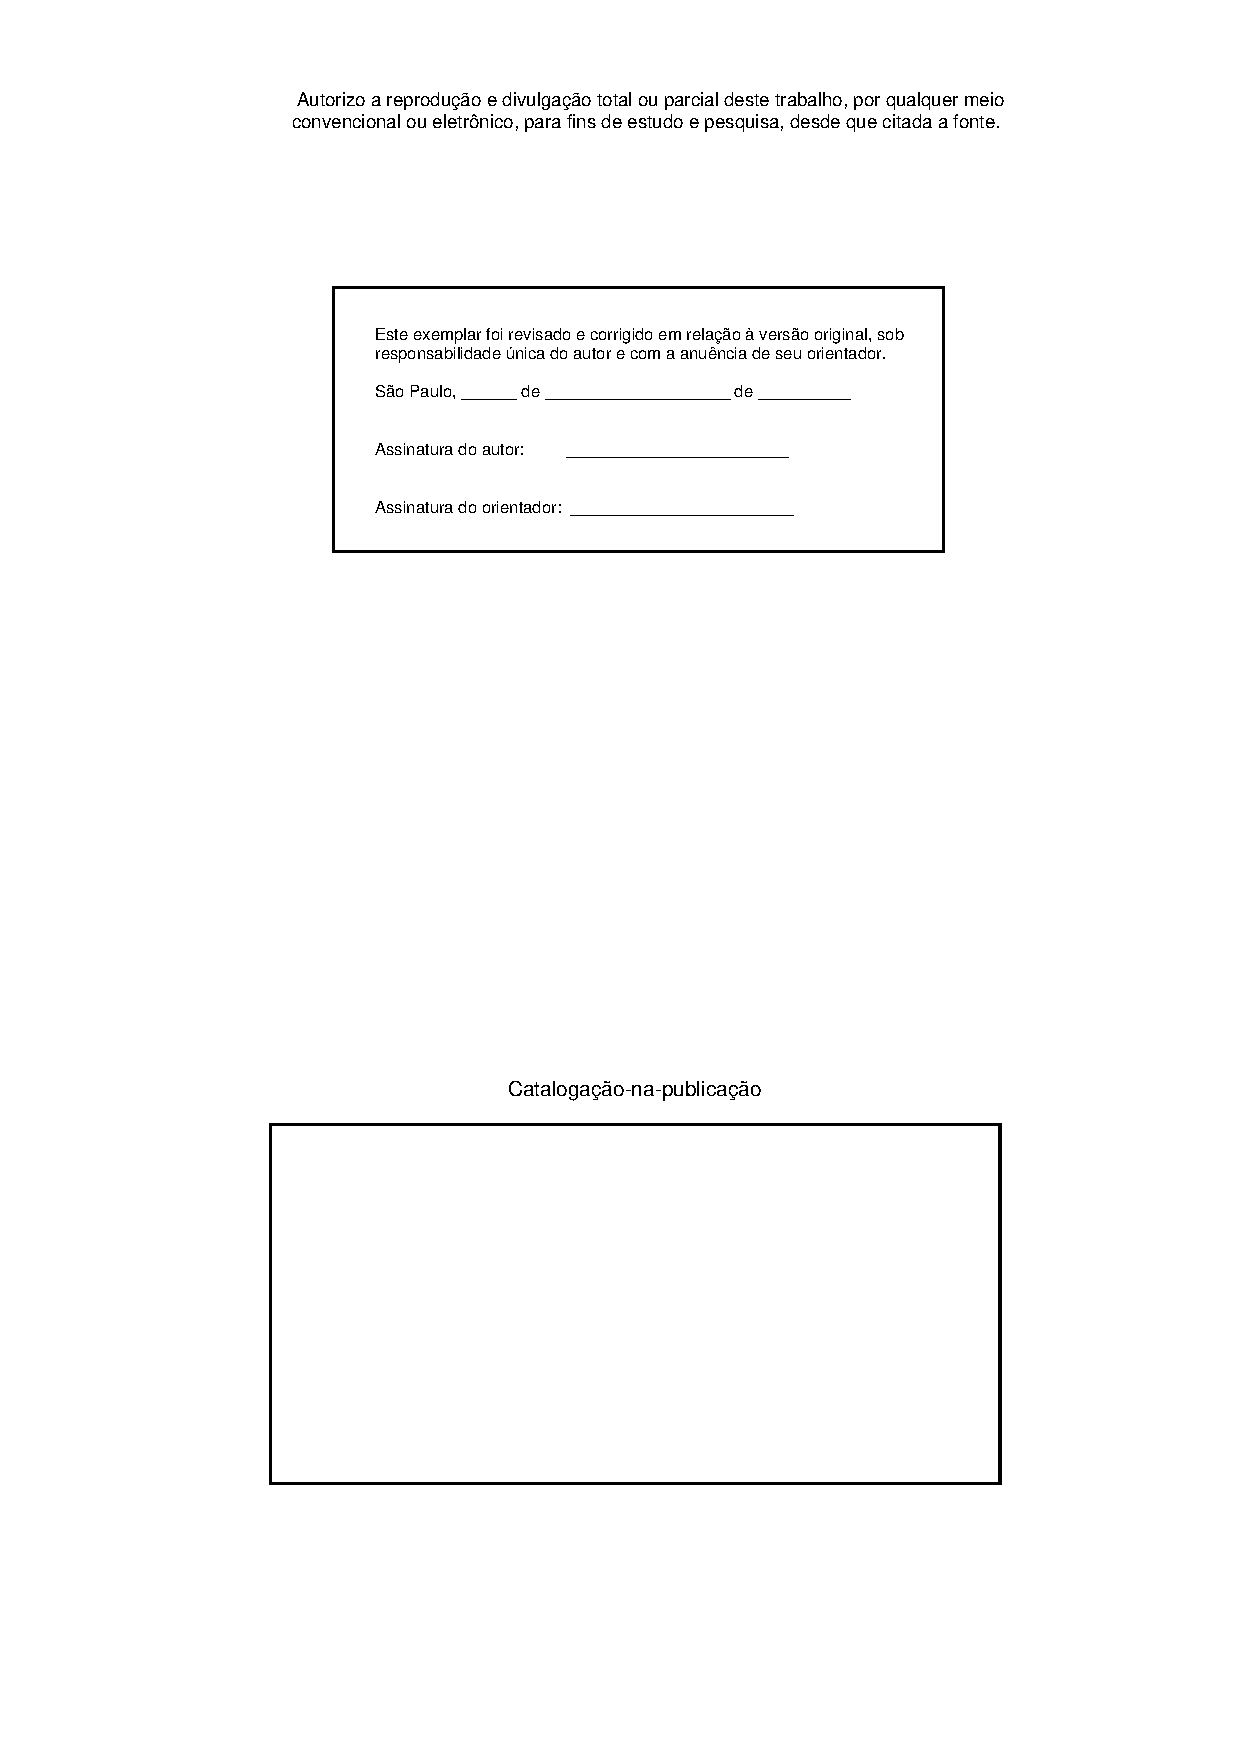
\includepdf[pages=1,scale=1,pagecommand={},linktodoc=true]{ficha.pdf}
\include{3-folhadeaprovacao}
\chapter*{Dedicatória}

\noindent Dedico este trabalho à Hihi e aos meus avós por terem cuidado de mim, ao meu irmão (o Di), e aos meus pais, Alfredo e Márcia.
\chapter*{Agradecimentos}

\noindent Agradecimentos texto.\\

Agradecemos ao Guilherme Migliati https://www.linkedin.com/in/guimigli?utm_source=share&utm_campaign=share_via&utm_content=profile&utm_medium=android_app foram essenciais para superar obstáculos no desenvolvimento do aplicativo, oferecendo suporte técnico, que permitiu a compilação dele.

\\

Além disso, a contribuição significativa do Dr.-Ing. Philippe Jardin https://www.linkedin.com/in/dr-ing-philippe-jardin-964733a3?utm_source=share&utm_campaign=share_via&utm_content=profile&utm_medium=android_app , que disponibilizou o simulador de OBD quando o Arthur ainda estava na Alemanha, ampliou consideravelmente as capacidades de teste do sistema. 

\chapter*{Epígrafe}

\noindent Epígrafe texto.\\
\pagestyle{plain}%%%%% Utilizar ESTILO PLAIN AQUI%%%%%%%
\chapter*{Resumo}

\noindent Este trabalho visa desenvolver a especificação de um sistema 'gimbal' open-source e open-hardware de baixo custo visando tornar esta tecnologia mais acessível. A demanda foi identificada pelo integrante Breno, ao perceber que os fabricantes cobravam preços muito altos inclusive por equipamentos amadores. \\
Especificamos o uso do microcontrolador ATMega328P por ser fácil de obter e estar presente na plataforma Arduino, ao qual a maioria dos usuários tem acesso. O OS escolhido é o armOS, por ter capacidades de tempo real, e que se comunicará com os periféricos: um giroscópio, acelerômetro, botões, servo-motores e LEDs.
\chapter*{Abstract}


\noindent Aiming to create a complementary platform for the driver and his car, this work used different sensors inside a car and those present in a cell phone to build a data compilation platform.\\
Data collection from the car was done through an OBD-II port, present in all vehicles manufactured from 2010 onwards in Brazil. Examples of data collected from a cell phone include information about the car's movement, such as geolocation and acceleration.\\
The collected data, in turn, was passed to the AWS cloud, for profile analysis of each driver.\\
% Each driver will be able to consult their personal data through a system with authentication, which is an exercise of implementation of security, an aspect fundamental to data protection.

%%%Comandos para criação automática das listas
%
\tableofcontents
\listoffigures
\listoftables

%%%Comandos para criar outras listas não suportadas pelo pacote ABNTex%%%
%
% \pretextualchapter{Lista de Símbolos}
% \begin{basedescript}{\desclabelstyle{\pushlabel}\desclabelwidth{6em}}
\item[$Z$] variavel aleatoria%
\item[$\mathbb{R}$] conjunto dos números reais%
\item[$t$] tempo contínuo%
\item[$n$] tempo discreto%
\item[$f(z)$] função densidade de probabilidade%
\item[$F(z)$] função de distribuição acumulada%
\item[$\sigma$] desvio padrão%
\item[$\mu$] média ou esperança matemática%
\item[$|\cdot|$] operador magnitude%
\item[$\nabla$] operador gradiente%
\end{basedescript}
% \newpage

\pretextualchapter{Lista de Abreviações}

\begin{basedescript}{\desclabelstyle{\pushlabel}\desclabelwidth{6em}}
% \item[{ANOVA}] \textit{Analysis of Variance}
\item[{API}] \textit{Application Programming Interface}
\item[{AWS}] \textit{Amazon Web Services}
\item[{IDE}] \textit{Integrated Development Environment}
\item[{IoT}] \textit{Internet of Things}
\item[{JSON}] \textit{Java Script Object Notation}
\item[{MVP}] \textit{Minimum Viable Product}
\item[{OBD-II}] \textit{On-board diagnostics}
\item[{PID}] \textit{Parameter Identifier}
\item[{RDS}] \textit{Amazon Relational Database Service}
\item[{RPM}] \textit{Revoluções por minuto}

% \item[{fda}] Função de distribuição acumulada%
% \item[{EMQ}] Erro médio quadrático%
\end{basedescript}
\newpage
%%%%%%%%%%%%%%%%%%%%%%%%%%%%%%%%%%%%%%%%%%%%%%%%%%%%%%%%%%%%%%%%%%%%

%Capítulos passam a ter páginas numeradas
%
\pagestyle{fancy}

%resseta os contadores de capítulo e seção
%
\renewcommand{\chaptermark}[1]{\markboth{#1}{}}
\renewcommand{\sectionmark}[1]{\markright{\thesection\ #1}}

%%%%%%%%%%%%%%NÃO LEMBRO O QUE FAZ, APARENTEMENTE NADA, TESTAR DEPOIS
%\fancyhf{}%
%\fancyhead[RO,LE]{\large\slshape\thepage}%
%\fancyhead[CE]{\large\slshape\leftmark}%
%\fancyhead[CO]{\large\slshape\rightmark}%


%%% Outros arquivos .tex. É acoselhável utilizar vários arquivos, pelo menos um por capítulo
\chapter{Introdução}\label{CAP:introducao}

Este documento consiste de um modelo basico para a producao de documentos academicos, seguindo as normas ABNT. 

Nao e abordado o estudo do LaTex neste template. Sugerimos a leitura do texto em \citeonline{Oetiker:1995}. O uso do LaTex e aconselhavel devido a sua qualidade grafica, facil referenciacao, criacao de listas, indices, referencias bibliograficas e escrita matematica profissional. Porem, nao e obrigatorio o uso deste template, apenas as orientacoes de formatação segundo as normas ABNT devem ser obrigatoriamente seguidas.

Uma observação em particular é a de que, no pacote ABNTex, as referências diretas devem utilizar o comando ``citeonline''. Referências indiretas utilizam o comando ``cite''.

Exemplo de citacao direta: Uma otima fonte de estudo para compreender o LaTex e apresentada por \citeonline{Oetiker:1995}. 

Exemplo de citação indireta: Existem boas fontes de pesquisa para entendimento do LaTex \cite{Oetiker:1995}, estas incluem documentação online disponível na web.

\section{Motivação}

Qual o perfil de direção de um motorista? Como categorizar os condutores segundo um critério claro?

Buscando responder essas perguntas e, consequentemente, entender as características de pessoas ao volante, este trabalho propõe-se a criar uma infraestrutura de captura e análise de dados em automóveis de uso pessoal.

As informações recolhidas serão armazenadas em uma plataforma de nuvem, protegidas por algum nível de segurança, implementado neste mesmo projeto e, por fim, serão analisadas para gerarem conclusões interessantes sobre o modo de dirigir de cada participante do estudo.
	
Uma pesquisa preliminar sobre o assunto revelou que já existe uma patente para um produto parecido; ela foi registrada em 2013 e avalia o desempenho de um motorista a partir de dados pré-coletados de parâmetros relevantes à condução do carro [REFERENCIA 1].

Visão lateral do carro proposto na patente.[IMAGEM, REF 1]

[CITAR OS TRABALHOS QUE JÁ FAZEM ISSO QUE EU DISSE]

\section{Objetivo}

Este trabalho procura analisar o comportamento de motoristas em situações diversas: no trânsito, em uma prova de direção ou em uma rodovia, por exemplo.

Para isso, fará uso da infraestrutura já presente em carros atuais, conforme pode ser visto na imagem a seguir, mas também pode complementá-la com mais equipamentos, caso seja necessário para o projeto.

[IMAGEM]
Sensores estão presentes em um carro atual na ordem de dezenas[2].

A coleta de dados será feita, a princípio, a partir de ensaios em carros reais feitos por uma quantidade seleta de pessoas, que pode ser expandida para resultados mais precisos na análise posterior.

Os dados coletados deverão ser passados para algum serviço de nuvem, usando conexão à Internet, caracterizando uma aplicação IoT.
	
Do lado da nuvem, será possível utilizar os dados de cada usuário de forma anônima, para diagnosticar o perfil do condutor e possivelmente gerar insights sobre como a pessoa poderia melhorar.
	
A plataforma poderá, após implementada, servir como base de dados para outros projetos futuros, que não farão parte deste TCC, por exemplo:

Prova de direção usando Inteligência Artificial: possível supressão da prova do Detran, avaliando o condutor ao longo das aulas práticas

Seguros de carro personalizados: valores mais altos para motoristas mais violentos

Classificação de motoristas de aplicativo: avaliação ponderada pela forma de dirigir

 
\section{Justificativa}
ROMEO e PIRES [GIT]
Pq o trabalho é importante?


\section{Organização do trabalho}
[ANTIGO "PROCUCAO CIENTIFICA"]

O padrão OBD-II foi uma extensão do padrão OBD-I, uniformizando esse tipo de conector em casos em geral, começando a ser adotado no Brasil a partir de 2010[4].

Nesse padrão de conexão e comunicação é definida uma interface por onde parâmetros internos a um carro podem ser monitorados.

As mensagens definidas pelo OBD-II têm cada uma um PID (parameter ID). O conjunto comum de PIDs de serviços que podem ser solicitados pela porta OBD-II e para que servem pode ser visto na tabela a seguir[REF 3].

[TABELA]

Service / Mode (hex)
Description
01
Show current data - I/M Monitors and Live Data
02
Show Freeze Frame (FF) Data
03
Show Stored Diagnostic Trouble Codes
04
Clear/Erase Diagnostic Trouble Codes and stored values
05
Test results, oxygen sensor monitoring (non CAN only)
06
Test results, other component/system monitoring (Test results, oxygen sensor monitoring for CAN only)
07
Show pending Diagnostic Trouble Codes (detected during current or last driving cycle)
08
Control operation of on-board component/system (EVAP)
09
Request Vehicle Information (VIN)
0A
Permanent Diagnostic Trouble Codes (DTCs) (Cleared DTCs)

É importante notar que os serviços do padrão OBD-II comuns a todos os carros sempre começam com o dígito zero (hexadecimal), por isso, serviços específicos de cada fabricante devem começam a partir do código 0x10.

[IMAGEM]

Posição da porta OBD-II em um carro[5].

Os dados que podem ser coletados de qualquer carros são explicitados na tabela abaixo[3]:

[TABELA]

Interessante notar que, embora não esteja representado na tabela, os PIDs 0x00, 0x20, 0x40, etc, ou seja, a cada 32 valores de PID, existe um parâmetro apenas para indicar quais entre os PIDs seguintes são fornecidos por aquele carro.

Esses PIDs de marcação, por assim dizer, utilizam 4 bytes para comunicar quais dos próximos PIDs estão disponíveis, utilizando cada bit como uma flag binária. 

Na imagem a seguir é possível visualizar como esse processo é feito, usando como exemplo o valor 0xBE1FA813 para representar os 4 bytes oferecidos[3].

[IMAGEM]


\section{Organização da tese}

\noindent \textbf{Capitulo \ref{CAP2}}: descricao...

\noindent \textbf{Capitulo \ref{CAP3}}: descricaoo...

\noindent \textbf{Capitulo \ref{CAP4}}: descricao...

\noindent \textbf{Capitulo \ref{CAP5}}: descricao...
\chapter{Aspectos conceituais}
\label{CAP2}

A seguir serão explicados os conceitos fundamentais que possibilitam a execução deste trabalho. 

% apresentar conceitos empregados e revisao da literatura (parte toerica do trab)

\section{O padrão OBD-II}

Criado na década de 1990 para gerar controle sobre as emissões de gás carbônico dos carros\textsuperscript{[5]}, hoje define um protocolo padronizado para comunicar parâmetros internos do veículo.
    
O padrão OBD-II foi uma extensão do padrão OBD-I, uniformizando esse tipo de conector em casos em geral, começando a ser adotado no Brasil a partir de 2010\textsuperscript{[4]}.

A comunicação é feita através de uma conexão física que normalmente pode ser encontrada abaixo do volante do motorista\textsuperscript{[5]}, conforme indicado pela figura \ref{fig:obd2_conn}.

Nesse padrão de conexão e comunicação é definida uma interface por onde parâmetros internos a um carro podem ser monitorados.

As mensagens definidas pelo OBD-II têm cada uma um PID (\textit{Parameter ID}). O conjunto comum de PIDs de serviços que podem ser solicitados pela porta OBD-II e para que servem pode ser visto na tabela \ref{Tb:tab1}\textsuperscript{[3]}.

\begin{table}[]
% \begin{adjustbox}{width=\textwidth}
\begin{tabular}{cc}
\rowcolor[HTML]{656565} 
{\color[HTML]{FFFFFF} Service / Mode (hex)} & {\color[HTML]{FFFFFF} Description}                                                                    \\
01                                          & Show current data - I/M Monitors and Live Data                                                        \\
02                                          & Show Freeze Frame (FF) Data                                                                           \\
03                                          & Show Stored Diagnostic Trouble Codes                                                                  \\
04                                          & Clear/Erase Diagnostic Trouble Codes and stored values                                                \\
05                                          & Test results, oxygen sensor monitoring (non CAN only)                                                 \\
06                                           & Test results, other component/system monitoring (Test results, oxygen sensor monitoring for CAN only) \\
07                                           & Show pending Diagnostic Trouble Codes (detected during current or last driving cycle)                 \\
08                                           & Control operation of on-board component/system (EVAP)                                                 \\
09                                          & Request Vehicle Information (VIN)                                                                     \\
0A                                          & Permanent Diagnostic Trouble Codes (DTCs) (Cleared DTCs)                                             
\end{tabular}
\end{table}

É importante notar que os serviços do padrão OBD-II comuns a todos os carros sempre começam com o dígito zero (hexadecimal), por isso, serviços específicos de cada fabricante devem começam a partir do código 0x10.

\begin{figure}[hp]
    \centering
    
    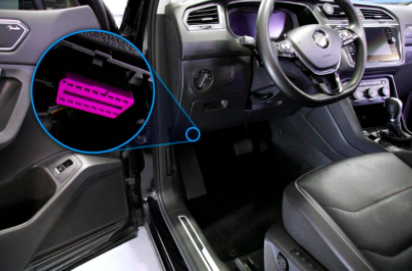
\includegraphics[]{figures/localizacao_obd2.png}
    
    \caption{Posição da porta OBD-II em um carro\textsuperscript{[5]}}
    
    \label{fig:obd2_conn}
\end{figure}

Os dados que podem ser coletados de qualquer carro são explicitados na tabela \ref{Tb:tab2}\textsuperscript{[3]}.

% Please add the following required packages to your document preamble:
% \usepackage[table,xcdraw]{xcolor}
% If you use beamer only pass "xcolor=table" option, i.e. \documentclass[xcolor=table]{beamer}
\begin{table}[]
\begin{tabular}{ccccccc}
\rowcolor[HTML]{C0C0C0} 
{\color[HTML]{FFFFFF} \textbf{PIDs(hex)}} & {\color[HTML]{FFFFFF} \textbf{PID(Dec)}} & {\color[HTML]{FFFFFF} \textbf{Data bytes returned}} & {\color[HTML]{FFFFFF} \textbf{Description}} & {\color[HTML]{FFFFFF} \textbf{Min value}} & {\color[HTML]{FFFFFF} \textbf{Max value}} & {\color[HTML]{FFFFFF} \textbf{Units}} \\
04                                         & 4                                        & 1                                                   & Calculated engine load                      & 0                                         & 100                                       & \%                                    \\
0C                                        & 12                                       & 2                                                   & Engine speed                                & 0                                         & 16,383.75                                 & rpm                                   \\
0D                                        & 13                                       & 1                                                   & Vehicle speed                               & 0                                         & 255                                       & km/h                                  \\
0F                                        & 15                                       & 1                                                   & Intake air temperature                      & -40                                       & 215                                       & °C                                    \\
1F                                        & 31                                       & 2                                                   & Run time since engine start                 & 0                                         & 65,535                                    & seconds                               \\
33                                        & 51                                       & 1                                                   & Absolute Barometric Pressure                & 0                                         & 255                                       & kPa                                   \\
46                                        & 70                                       & 1                                                   & Ambient air temperature                     & -40                                       & 215                                       & °C                                    \\
47                                        & 71                                       & 1                                                   & Absolute throttle position B                & 0                                         & 100                                       & \%                                    \\
49                                        & 73                                       & 1                                                   & Accelerator pedal position D                & 0                                         & 100                                       & \%                                    \\
51                                        & 81                                       & 1                                                   & Fuel Type                                   & -                                         & -                                         & -                                     \\
52                                        & 82                                       & 1                                                   & Ethanol fuel \%                             & 0                                         & 100                                       & \%                                    \\
5A                                        & 90                                       & 1                                                   & Relative accelerator pedal position         & 0                                         & 100                                       & \%                                    \\
5B                                        & 91                                       & 1                                                   & Hybrid battery pack remaining life          & 0                                         & 100                                       & \%                                    \\
5C                                        & 92                                       & 1                                                   & Engine oil temperature                      & -40                                       & 210                                       & °C                                    \\
5D                                        & 93                                       & 2                                                   & Fuel injection timing                       & -210.00                                   & 301992                                    & °                                     \\
5E                                        & 94                                       & 2                                                   & Engine fuel rate                            & 0                                         & 3212.75                                   & L/h                                   \\
61                                        & 97                                       & 1                                                   & Driver's demand engine - percent torque     & -125                                      & 130                                       & \%                                    \\
62                                        & 98                                       & 1                                                   & Actual engine - percent torque              & -125                                      & 130                                       & \%                                    \\
63                                        & 99                                       & 2                                                   & Engine reference torque                     & 0                                         & 65,535                                    & Nm                                    \\
64                                        & 100                                      & 5                                                   & Engine percent torque data                  & -125                                      & 130                                       & \%                                    \\
70                                        & 112                                      & 10                                                  & Boost pressure control                      & -                                         & -                                         & -                                     \\
83                                        & 131                                      & 9                                                   & NOx sensor                                  & -                                         & -                                         & -                                     \\
8E                                        & 142                                      & 1                                                   & Engine Friction - Percent Torque            & -125                                      & 130                                       & \%                                   
\end{tabular}
\end{table}

Interessante notar que, embora não esteja representado na tabela, os PIDs 0x00, 0x20, 0x40, etc, ou seja, a cada 32 valores de PID, existe um parâmetro apenas para indicar quais entre os PIDs seguintes são fornecidos por aquele carro.

Esses PIDs de marcação, por assim dizer, utilizam 4 bytes para comunicar quais dos próximos PIDs estão disponíveis, utilizando cada bit como uma \textit{flag} binária. 

Na figura \ref{fig:bitwise_obd2} é possível visualizar como esse processo é feito, usando como exemplo o valor \textit{0xBE1FA813} para representar os 4 bytes oferecidos\textsuperscript{[3]}.

\begin{figure}[hp]
    \centering
    
    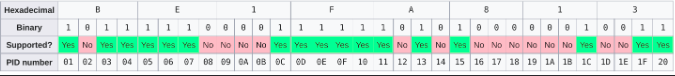
\includegraphics[scale=0.7]{figures/tabela_dados_disponiveis.png}
    
    \caption{Divisão bit a bit da mensagem OBD-II informando os serviços disponíveis\textsuperscript{[3]}}
    
    \label{fig:bitwise_obd2}
\end{figure}

A coleta de fato dos dados relevantes será feita por uma aplicação desenvolvida \textit{a priori} que já é capaz de comunicar-se corretamente com a interface OBD.

Essa aplicação acelerará a criação da infraestrutura proposta por este trabalho, uma vez que pula o primeiro passo da estratégia \textit{bottom-up} que deverá permear o projeto.

\section{Transmissão de dados}

A implementação da transmissão \textit{Bluetooth} neste projeto de compilação de dados oferece uma solução eficaz para a comunicação entre os produtor e consumidor de dados. 

Ao utilizar essa tecnologia, os dados de rastreamento podem ser transmitidos de forma sem fio e em tempo real para dispositivos equipados com \textit{Bluetooth}, como \textit{smartphones}, que são o foco deste trabalho.

A abordagem \textit{wireless} proporciona uma conectividade mais flexível, eliminando a necessidade de cabos físicos e simplificando a integração do sistema. A baixa energia do \textit{Bluetooth} permite uma transmissão eficiente de dados, minimizando o impacto no consumo de bateria dos dispositivos móveis.

Além disso, a transmissão \textit{Bluetooth} possibilita a interação direta entre o sistema de geração e os usuários, permitindo a visualização em tempo real de informações de condução.

Essa integração sem fio não apenas aprimora a experiência do usuário, mas também amplia as possibilidades de interatividade e controle, tornando o sistema mais acessível e fácil de usar.

 \begin{figure}[hp]
    \centering
    
    
\includegraphics[scale=0.4]{figures/bluetooth.png}
    
    \caption{Logo do Bluetooth.}
    
\end{figure}

\section{Armazenamento em nuvem}
Provedoras como a Amazon e a Azure (Microsoft) oferecem serviços de nuvem que podem ser usados para este projeto \textsuperscript{[10, 11]}. Neste trabalho, optou-se pelo serviço da AWS, uma vez que um dos integrantes do grupo já tinha familiaridade com o serviço.

A integração do aplicativo Android com o Amazon RDS (Relational Database Service) da AWS oferece uma solução eficiente e escalável para o armazenamento de dados. 

Utilizando o RDS, os dados coletados, como informações de localização, velocidade e aceleração, podem ser armazenados em bancos de dados relacionais, proporcionando alta disponibilidade, segurança e desempenho otimizado. 

A flexibilidade do Amazon RDS permite a escolha de diferentes motores de banco de dados, como MySQL, PostgreSQL, ou SQL Server, adequando-se às necessidades específicas do sistema.

Os usuários poderão transmitir informações para a nuvem a qualquer momento, desde que seus carros estejam ligados e conectados à internet. O volume de dados recebidos no sistema é, portanto, variável e por isso fez sentido que o serviço de nuvem contratado siga o modelo \textit{on-demand}. A figura \ref{figure:custo_aws_inicial} mostra o custo calculado no serviço da AWS RDS.

\begin{figure}[hp]
    \centering
    
    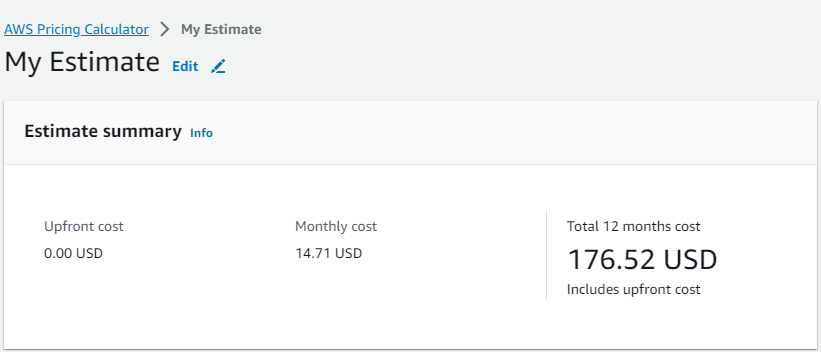
\includegraphics[scale=0.8]{figures/custo_aws_inicial.PNG}
    \caption{Custo da AWS.}
    \label{figure:custo_aws_inicial}
    
\end{figure}

A região do Leste da Virgina é conhecida por ter uma alta densidade de \textit{data centers}. Isso resulta em eficiência operacional e redução de custos.

A instância escolhida foi a \textbf{db.t3.micro}. Ela é uma instância de banco de dados pequena, sendo adequada para cargas de trabalho leves. Essa instância é comumente usada para ambientes de desenvolvimento, testes ou pequenas aplicações que não exigem muitos recursos.

Um RDS Proxy é um serviço que facilita a escalabilidade e a alta disponibilidade para as conexões de banco de dados. Ele ajuda a melhorar o desempenho e a segurança ao gerenciar as conexões entre seus aplicativos e instâncias de banco de dados RDS. Isso é especialmente útil em ambientes onde há flutuações na carga de trabalho. Como se trata de um protótipo, não há preocupações com carga de trabalho. Logo, essa opção não foi escolhida.

Também não há necessidade de ter um ambiente de zona de disponibilidade múltipla para garantir escalabilidade, pois haveria custo adicional. Por isso, a instância RDS foi configurada para o modo Single-AZ. E a capacidade de armazenamento foi 20 GB.


\begin{table}[]
\begin{tabular}{|ll|}
\hline
\multicolumn{1}{|l|}{\textbf{Região}}                 & Virgínia     \\ \hline
\multicolumn{1}{|l|}{}                                &              \\ \hline
\multicolumn{2}{|c|}{\textbf{Especificação das instancias do MySQL}} \\ \hline
\multicolumn{1}{|l|}{Quantidade de Instancias MYSQL}  & 1            \\ \hline
\multicolumn{1}{|l|}{tipo da instancia}               & db.t3.micro  \\ \hline
\multicolumn{1}{|l|}{vCPU}                            & 2            \\ \hline
\multicolumn{1}{|l|}{Memória}                         & 1GiB         \\ \hline
\end{tabular}
\end{table}
\chapter{Metodologia do trabalho}
\label{CAP3}

Esta seção trata das fases do trabalho: como deverão ser executadas e em que sequência.

% descrever fases do trab: concepcao, projeto, implementacao, testes
% (falar com o prof)


\section{OBD-II / coleta dos dados}
Já existe uma plataforma aceleradora desenvolvida no GitHub que consegue comunicar-se com o veículo através do protocolo OBD-II\textsuperscript{[12]}. Esse outro projeto, já implementa o protocolo OBD-II e implementa uma interface gráfica básica para mostrar os dados fornecidos pelo carro.

Na imagem \ref{fig:git_obd_interface} é possível ver alguns dos dados já previstos por essa plataforma.

\begin{figure}[hp]
    \centering
    
    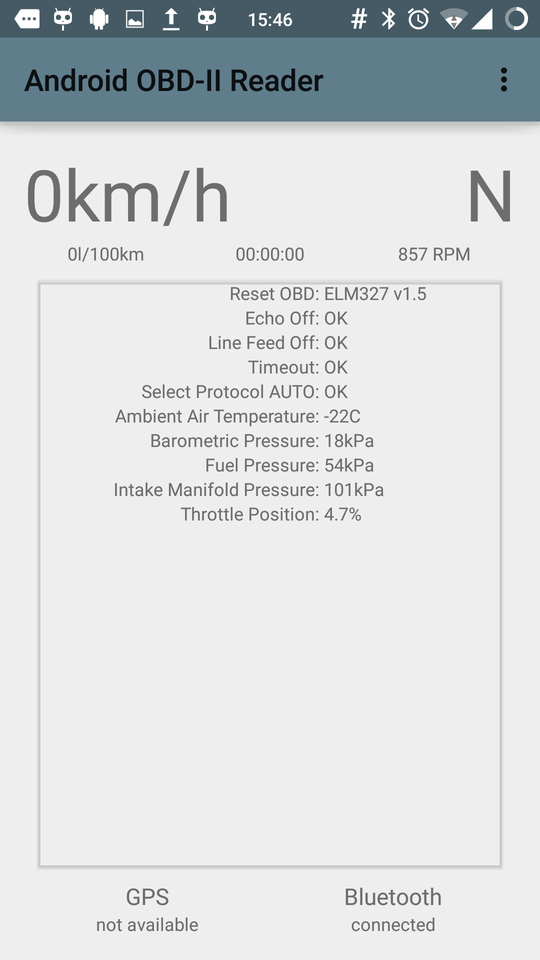
\includegraphics[scale=0.3]{figures/git_obd_interface.png}
    
    \caption{Interface básica com porta OBD-II\textsuperscript{[12]}.}
    
    \label{fig:git_obd_interface}
\end{figure}

Nesta fase do desenvolvimento caracteriza-se pela adaptação do aplicativo para que possa atender aos requisitos do projeto.

Primeiro, será preciso entender a estrutura e o funcionamento do código através da IDE do \textit{Android Studio}, que foi por onde essa plataforma foi originalmente desenvolvida.

Complementarmente ao que for fornecido pela porta OBD, poderão ser usados também dados externos ao carro, como os de navegação fornecidos pelo Waze através dos próprios motoristas que passam em cada via\textsuperscript{[13]}, informações de localização via GPS e também a aceleração desempenhada pelo carro durante seu trajeto.

Essas outras informações serão de grande importância na fase final do projeto, de análise dos dados coletados.

A viabilidade dessa última parte, de utilizar dados fornecidos pelo celular, pode ser vista em um estudo publicado em 2014 no \textit{site} da IEEXplore\textsuperscript{[15]}.

Esse artigo utiliza parâmetros de movimentos bruscos do carro, e.g. mudança de faixa, e a velocidade do veículo para classificar o motorista como mais ou menos agressivo, a partir de um \textit{score} chamado de \textit{driver safety index}.

A imagem \ref{fig:sudden_acc_car} ilustra como essa análise pode ser feita, mas sem entrar em detalhes técnicos de como isso é possível.

\begin{figure}[hp]
    \centering
    
    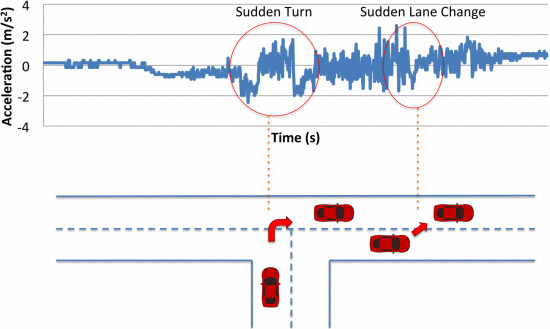
\includegraphics[scale=0.6]{figures/sudden_acc_car.jpg}
    
    \caption{Correspondência entre variações de aceleração e movimentos relativos do carro\textsuperscript{[15]}.}
    
    \label{fig:sudden_acc_car}
\end{figure}

\section{Transferência de dados para a nuvem e estruturação}
Uma vez que a plataforma aceleradora esteja adaptada ao novo sistema, os dados coletados deverão ser passados para uma plataforma remota, que armazenará os dados brutos coletados para depois serem processados e analisados na fase seguinte.

O \textit{pipeline} de captura e armazenamento de informações estará consolidado quando for definida uma estrutura fixa para o processamento dos dados crus e o formato em que serão guardados na nuvem.

Isso poderá ser feito fixando-se uma especificação básica de arquivos JSON que deverá ser seguida pelas APIs que fizerem uso do banco de dados da nuvem.

\section{Geração dos dados}
O sistema poderá ser usado assim que os protocolos e estruturas básicos de comunicação tiverem sido definidos. 

Neste momento serão necessários voluntários para fornecer dados ao sistema e quanto mais pessoas puderem participar, melhor será a análise de perfil feita ao fim do projeto.

\section{Visualização dos dados}
Uma aplicação Web básica para visualização dos dados individuais de cada motorista deverá ser implementada.

Essa plataforma deverá permitir que apenas usuários autorizados acessem suas próprias informações. Para isso, algum sistema de segurança deverá ser implementado.

Na área logada do motorista, será possível visualizar estatísticas básicas acerca do que foi coletado pela porta OBD.

A princípio, serão apresentados bem poucos dados, os quais serão definidos assim que o sistema for um pouco mais palpável. 

\section{Análise dos dados}
Finalmente, com toda a infraestrutura do projeto já funcional, será possível gerar estatísticas relevantes sobre cada motorista.

Quais parâmetros serão gerados ou que análise será feita objetivamente ainda será objeto de discussão no projeto, mas uma das ideias primárias era tentar definir métricas que diferenciem um motorista do outro, isto é, que definam o seu perfil de condução.

Conforme o artigo citado anteriormente (\textit{Driver behaviour profiling using smartphone sensory data in a V2I environment}\textsuperscript{[15]}), é possível usar métricas de movimentação brusca do carro para classificar motoristas segundo a segurança de sua direção.

Mais especificamente, o estudo determina quatro tipos de condutores: muito cautelosos, cautelosos, agressivos e muito agressivo\textsuperscript{[15]}.

A classificação depende basicamente de quantos movimentos bruscos são feitos e em que situações eles ocorrem. Isso significa que em um ponto de maior convergência de estradas, por exemplo, haverá maior penalidade para o \textit{driver safety index} que em um local de menos movimento ou.

Dessa forma, esse estudo procura ranquear melhor os motoristas que têm menos probabilidade de gerar acidentes.
\chapter{Especificação de requisitos do trabalho}

\label{CAP4}


% definir técnicas, processos e sistemas, procedimentos que vão compor o sistema

Neste capítulo serão descritas as necessidades básicas levantadas para que o projeto funcione como esperado.

Na figura \ref{fig:class_diagram} pode ser visto o diagrama de classes que define o sistema como um todo.

\begin{figure}[hp]
    \centering
    
    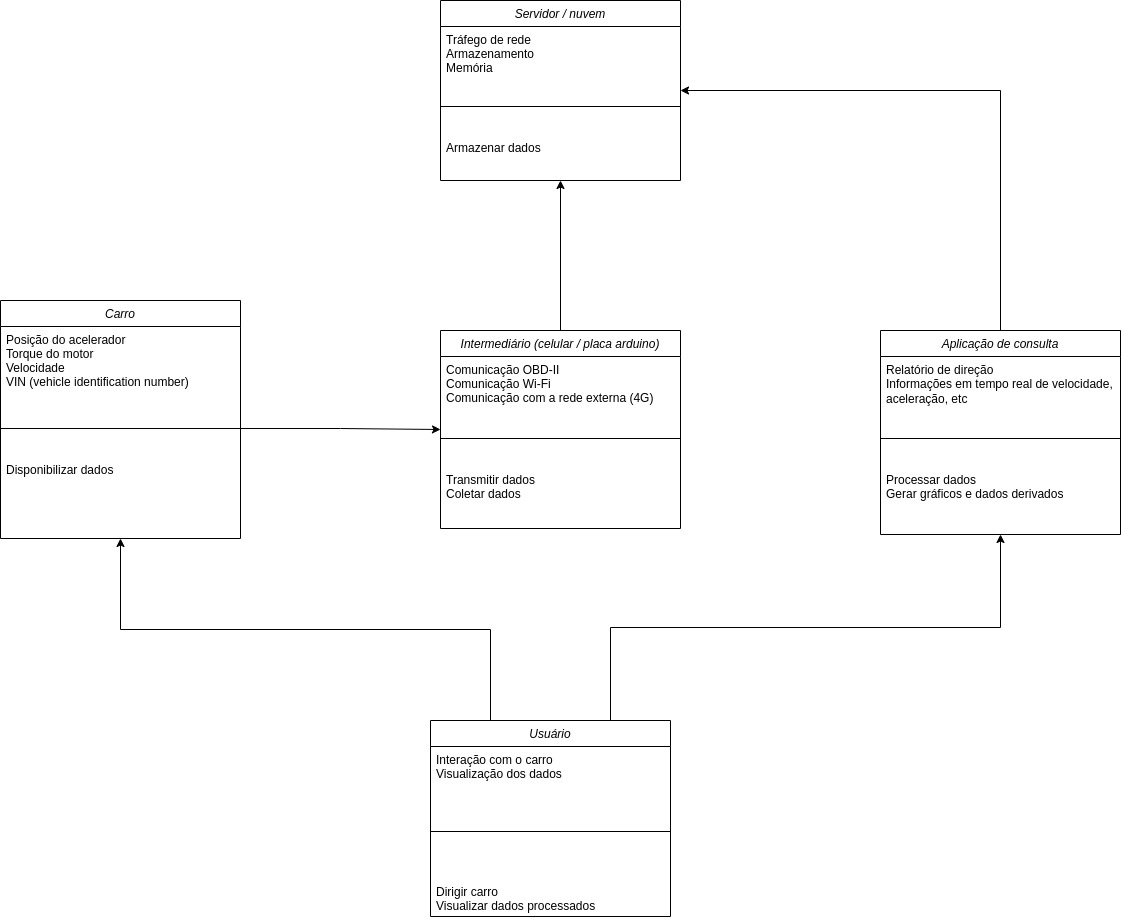
\includegraphics[scale=0.4]{figures/coleta_dados_carro}
    
    \caption{Diagrama de classes com visão mais abstrata do sistema}
    
    \label{fig:class_diagram}
\end{figure}

\section{Requisitos funcionais}
\begin{itemize}
    \item \textbf{Comunicação OBD-II:} fará comunicação com a interface do carro, requisitando apenas as informações definidas, durante o projeto, como relevantes.
    
    \item \textbf{Interface com celular ou módulo de \textit{WiFi}:} deverá estabelecer conexão sem fio com a internet, usando a tecnologia 4G, além de aproveitar-se dos dados de GPS e de aceleração fornecidos pelo celular.
    
    \item \textbf{Plataforma de recepção na nuvem:} utilizando um serviço de armazenamento ainda a ser definido, os dados brutos coletados do carro, do celular (GPS e acelerômetro) e da internet (\textit{Waze}, por exemplo, para informações de tráfego em cada via), assim como as informações depois já processadas, serão todos armazenados na plataforma de \textit{cloud} escolhida.
    
    \item \textbf{\textit{Dashboard} básico informativo:} haverá uma plataforma \textit{Web} que disponibilizará algumas informações básicas para o usuário; deverá ser uma mistura dos dados crus provindos diretamente do carro e também os processados posteriormente, para geração de novas informações também relevantes.
\end{itemize}

\section{Requisitos não-funcionais}

\begin{itemize}
    \item \textbf{Conexão contínua com a internet:} caso a conexão pare por muito tempo, a análise dos dados coletados pode ser prejudicada, além de gerar desconfiança por parte do usuário não havendo garantia de que o sistema é consistente.
    
    \item \textbf{Interface sem reconexão manual com a internet:} se o sistema desligar, a conexão com o celular e com a internet devem ser estabelecidas sem interferência do usuário assim que for ligado novamente; em outras palavras, o sistema deve ser o mais \textit{plug and play} possível.
    
    \item \textbf{Informações relevantes e corretas:} os dados apresentados no \textit{dashboard} precisam ter sentido para o usuário; informações palpáveis como velocidade, aceleração e trajeto percorrido são as únicas que devem chegar até o usuário final, e também precisam passar por algum tipo de "filtro de plausibilidade", para, mais uma vez, não se perder a confiança de quem usará o sistema, apresentando valores \textit{outliers} coletados. 
    
    \item \textbf{Memória e armazenamento em nuvem suficientes:} seja oferecendo espaço ilimitado para o usuário ou definindo um tamanho máximo que pode ser usado, deve ficar claro para o usuário quando e se os seus dados serão apagados do sistema; uma possibilidade seria apagar as informações mais velhas sempre que falte armazenamento.
    
    \item \textbf{Segurança de dados:} pessoas não-autorizadas não pode ter acesso aos dados coletados no veículo de cada usuário.
\end{itemize}

% \subsection{}
% \subsection{}
% \subsection{}



\chapter{Desenvolvimento do trabalho}

% Apresentar os resultados das fases que transformam
% os requisitos em produtos finais.
% • A estrutura desse capítulo depende do processo de
% desenvolvimento do trabalho.
% • A organização e as seções desse capítulo devem ser
% definidas juntamente com o orientador.

Este capítulo tem como objetivo explicitar quais foram as decisões de projeto que foram tomadas ao longo do desenvolvimento do sistema.

\section{Justificativas das métricas escolhidas}

A escolha das métricas para o desenvolvimento desse projeto foi determinante para avaliar e interpretar resultados com precisão e, como era o objetivo do trabalho, avaliar o perfil de motoristas.

Uma conversa com um funcionário da empresa Porto Seguro foi determinante para ratificar a relevância das métricas definidas. Essa conversa pode ser vista no Apêndice 7.1 deste documento.

\subsection{Gasto do motor a partir do RPM}

Em um motor de combustão interna, o RPM indica a velocidade com que os pistões se movem para cima e para baixo no cilindro. O controle preciso do RPM é essencial para otimizar a eficiência do motor e a entrega de potência, sendo um indicador chave para os motoristas ajustarem suas velocidades de condução.

A figura \ref{fig:rpmxpotencia} mostra que a potência gasta por um motor aumenta quando a rotação dele também ascende\textsuperscript{[28]}. 
 
Dado que a amplitude de tais ondulações (alto RPM) reduz ao longo da vida útil de um pistão, deve-se levar em consideração o efeito do desgaste ao especificar a rugosidade superficial da saia do pistão. Caso contrário, o pistão poderá vir a engripar no cilindro por não ser capaz
de reter óleo em sua superfície \textsuperscript{[40]}.

Durante o funcionamento do motor, a biela fica sujeita a forças de compressão muito elevadas, provenientes da fase de expansão do cilindro e a forças de tração, nas fases de admissão do motor. Sendo assim, as bielas são mais solicitadas nas condições de plena carga e de elevadas rotações do motor\textsuperscript{[40]}.


 \begin{figure}[hp]
    \centering
    
    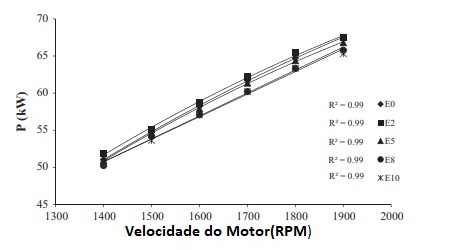
\includegraphics[scale= 1]{figures/rpmxpotencia.jpeg}
    
    \caption{Potência gasta pelo motor em função de sua rotação.}
    
    \label{fig:rpmxpotencia}
\end{figure}

\subsection{Trajetos e rotas perigosas}

A relação entre rotas perigosas, marcadas por assaltos e roubos de carros e o perfil do motorista torna-se um elemento crítico na gestão da segurança. A escolha da rota desempenha um papel significativo na mitigação desses perigos. 

Motoristas que optam por passar frequentemente por áreas consideradas de alto risco podem estar mais suscetíveis a incidentes indesejados. Portanto, compreender o perfil do motorista em relação a essas rotas perigosas é importante para a implementação de estratégias eficazes de prevenção. 

A conscientização dos motoristas sobre áreas de risco pode contribuir para um comportamento mais prudente ao planejar e seguir rotas.

Na cidade de São Paulo, locais como Paulista, Augusta e Sé possuem altos índices de furtos\textsuperscript{[34]}. A figura \ref{fig:mapa_calor_violencia} mostra as áreas com maior índice de assaltos na metrópole.

\begin{figure}[hp]
    \centering
    
    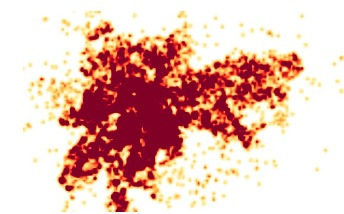
\includegraphics[scale= 1]{figures/mapa_calor_violencia.jpeg}
    
    \caption{Mapa de calor dos incidentes criminais na cidade de São Paulo. Com atenção, é possível ver o contorno da cidade nesta imagem.}
    \label{fig:mapa_calor_violencia}
    
\end{figure}

A figura \ref{fig:mapa_risco_acc_rpm} ilustra alguns dos metadados que podem ser gerados com a análise dos dados obtidos. De forma semelhante, as tabelas \ref{Tb:tab_fracao_acc} e \ref{Tb:tab_fracao_perigo} detalham quanto por cento do tempo o motorista passa acelerando o carro e também a fração de tempo passada em cada região da cidade, respectivamente. Ambas as métricas são subdivididas em três categorias: baixo, médio e alto risco.

\begin{table}[]

    \caption{Exemplo de análise qualitativa da aceleração do carro durante a coleta de dados.}
    \label{Tb:tab_fracao_acc}
    \centering

    \begin{center}
    % \begin{tabular}{lllll}
    % \begin{adjustbox}{width=\textwidth}
        \begin{tabular}{ccc p{6cm} ccc}
            % \rowcolor[HTML]{C0C0C0}
            % \cline[2-3]
            
            \multicolumn{1}{l}{}  & \multicolumn{1}{|l}{
                \textbf{Fração do tempo com cada tipo de aceleração}
            }  \\
            
            % \cellcolor[HTML]{C0C0C0} \textbf{Fração do tempo com cada tipo de aceleração}}  \\

            \hline
            
            \multicolumn{1}{l|}{Aceleração normal}  & \multicolumn{1}{|l}{0,00\%}    \\

            \hline
            
            \multicolumn{1}{l|}{Aceleração média}  & \multicolumn{1}{|l}{55,30\%}    \\

            \hline
            
            \multicolumn{1}{l|}{Aceleração muito alta}  & \multicolumn{1}{|l}{44,70\%}    \\
        \end{tabular}
    % \end{adjustbox}
    \end{center}
\end{table}

% \input{tabelas/tab_fracao_rpm}
\begin{table}[]

    \caption{Exemplo de análise qualitativa de por onde o carro passa durante a coleta de dados.}
    \label{Tb:tab_fracao_perigo}
    \centering

    \begin{center}
    % \begin{tabular}{lllll}
    % \begin{adjustbox}{width=\textwidth}
        \begin{tabular}{ccc p{6cm} ccc}
            % \rowcolor[HTML]{C0C0C0}
            % \cline[2-3]
            
            \multicolumn{1}{l}{}  & \multicolumn{1}{|l}{
                \textbf{Fração do tempo passada em cada tipo de lugar}
            }  \\
            
            % \cellcolor[HTML]{C0C0C0} \textbf{Fração do tempo com cada tipo de aceleração}}  \\

            \hline
            
            \multicolumn{1}{l|}{Baixo risco}  & \multicolumn{1}{|l}{54,55\%}    \\

            \hline
            
            \multicolumn{1}{l|}{Médio risco}  & \multicolumn{1}{|l}{45,45\%}    \\

            \hline
            
            \multicolumn{1}{l|}{Alto risco}  & \multicolumn{1}{|l}{44,70\%}    \\
        \end{tabular}
    % \end{adjustbox}
    \end{center}
\end{table}


% \begin{figure}[hp]
%     \centering
    
%     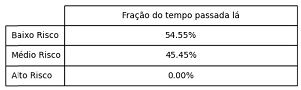
\includegraphics[scale= 1]{figures/tabela_fracao1.jpg}
    
%     \caption{Potência versus velocidade do motor.}
    
    
% \end{figure}

\begin{figure}[hp]
    \centering
    
    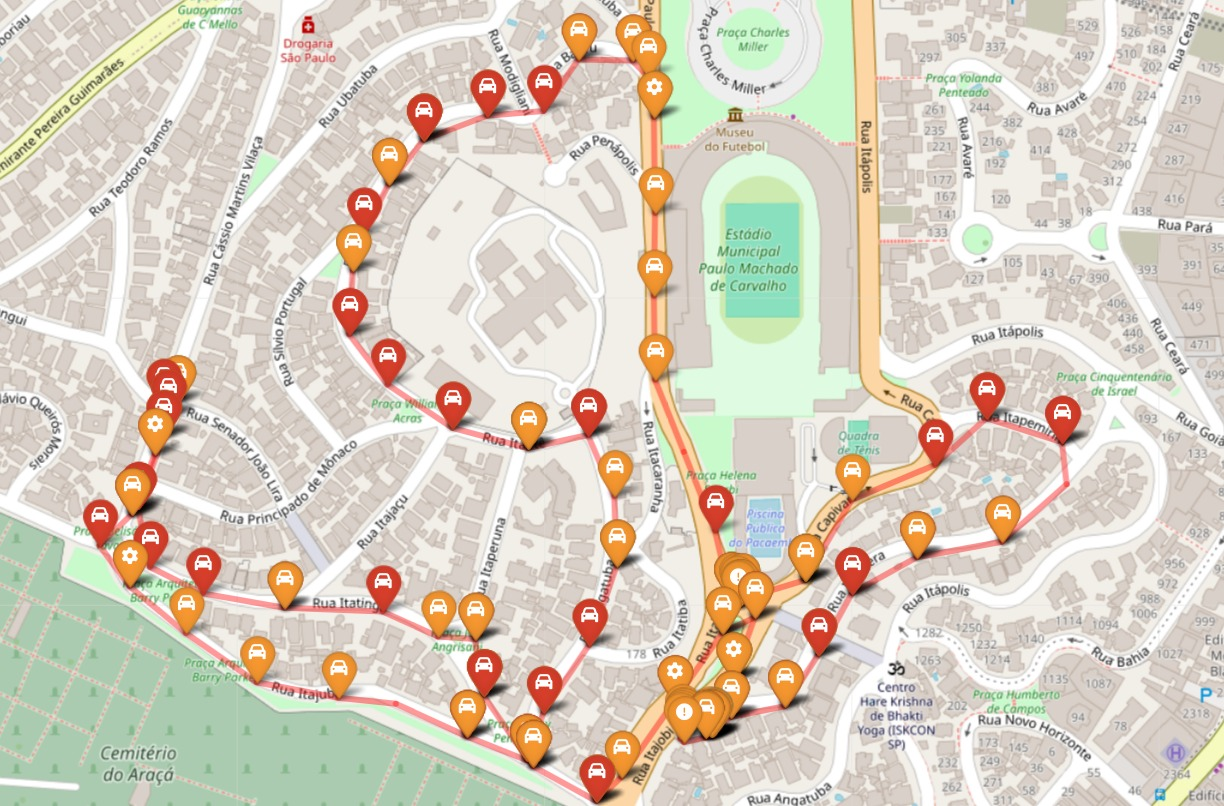
\includegraphics[scale=0.25]{figures/mapa_risco_acc_rpm.jpeg}
    
    \caption{Mapa de risco em acelerações (símbolo de carro) e valores de RPM (símbolo de engrenagem).}
    
    \label{fig:mapa_risco_acc_rpm}
\end{figure}


% \begin{figure}[hp]
%     \centering
    
%     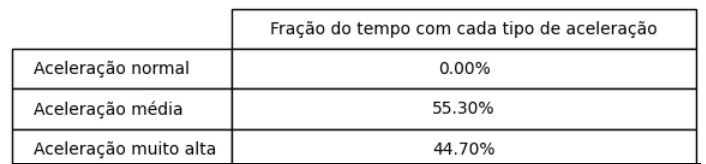
\includegraphics[scale= 0.85]{figures/tabela_2.jpg}
    
%     \caption{Fração da aceleração.}
    
%     \label{fig:tab1}
% \end{figure}

% \begin{figure}[hp]
%     \centering
    
%     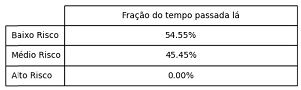
\includegraphics[scale= 0.95]{figures/tabela_fracao1.jpg}
    
%     \caption{Tipo de risco.}
    
%     \label{fig:tab2}
% \end{figure}


A construção dessa figura foi feita graças a uma base de dados encontrada no site Kaggle\textsuperscript{[33]}, conhecido por hospedar \textit{Jupyter Notebooks} analisando certos conjuntos de informações.

Embora a descrição do \textit{dataset} mencione que os dados referem-se só a São Paulo (o que já gera ambiguidade entre cidade e estado), existem lá registros de Curitiba, Rio de Janeiro e Pará também.

Importante mencionar que, devido ao tamanho dessa base de dados, de 12899 linhas, foi preciso pensar-se em como comparar os dados nela contidos com cada um dos registros de GPS fornecidos pelo \textit{app} sem que o desempenho dessa análise fosse comprometido.

Para tal, as coordenadas geográficas da planilha foram indexadas conforme indicado no código-fonte presente no Apêndice 7.5.

Alguns números mágicos (constantes sem derivação algorítmica), que foram utilizados nesse código, levaram em consideração a equivalência entre graus e quilômetros da Terra e as distâncias entre os pontos mais a sul, norte, leste e oeste do Brasil\textsuperscript{[35, 36]}.

A ideia dessa indexação é dividir o mapa em \textit{chunks}, os quais limitam o trabalho computacional a um subconjunto dos dados. Cada \textit{chunk} é um quadrado de lado 500m, o que obriga o programa a olhar alguns blocos adjacentes ao onde está a coordenada cuja segurança quer-se verificar.

% \begin{figure}[hp]
%     \centering
    
%     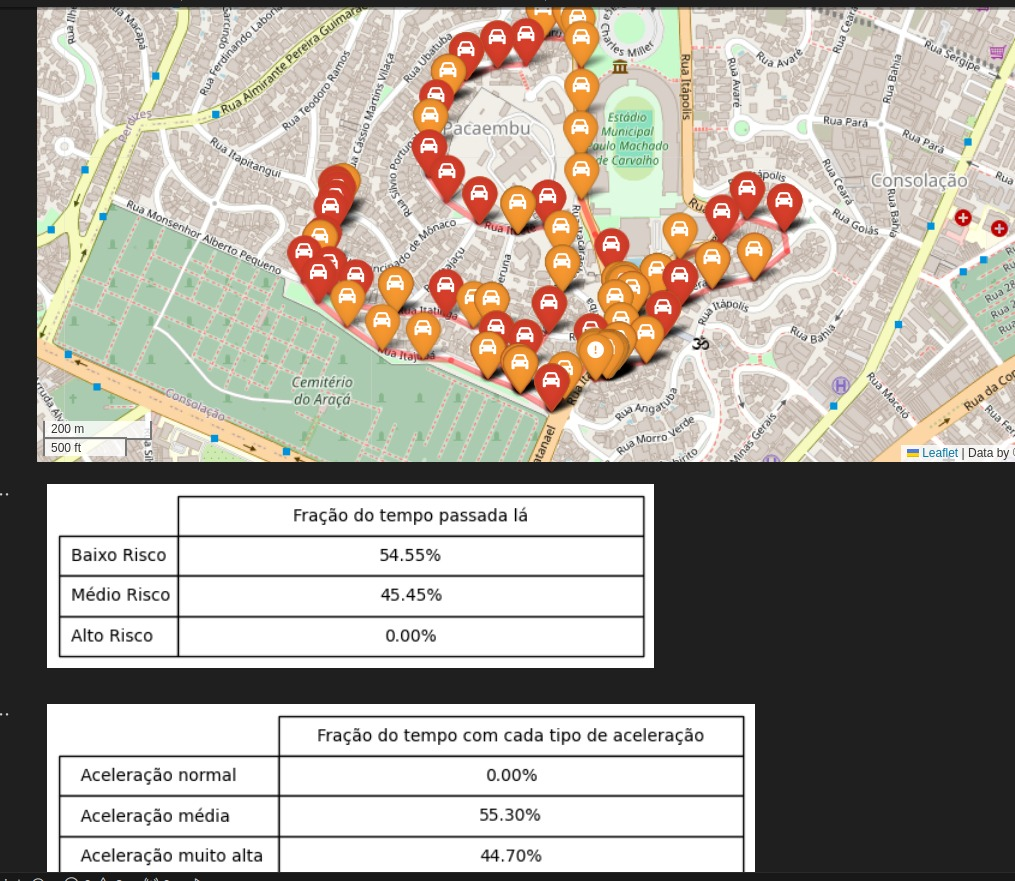
\includegraphics[scale=0.8]{figures/rotas_altorisco.jpeg}
    
%     \caption{}
    
%     \label{fig:rotas_altorisco}
% \end{figure}

 
\section{Tecnologias utilizadas}
O projeto definiu algumas tecnologias de base para serem usadas durante o desenvolvimento de cada fase dele.

    \subsection{Amazon Web Services}

    A escolha da AWS para o projeto é fundamentada em três pilares essenciais: escalabilidade, segurança e viabilidade econômica. 
    
    A capacidade desse serviço de nuvem de se adaptar dinamicamente às demandas do sistema assegura uma infraestrutura flexível, capaz de lidar eficientemente com variações na carga de trabalho. 
    
    Além disso, a reputação consolidada da Amazon em termos de segurança oferece uma base robusta para proteção dos dados e operações. 
    
    Por fim, a viabilidade econômica se destaca, uma vez que a AWS disponibiliza uma variedade de serviços e modelos de precificação que se alinham de maneira eficaz às necessidades do projeto, otimizando custos operacionais.

    É evidente que todas essas vantagens só são concretizadas caso os implementadores do sistema façam uso de toda a funcionalidade da nuvem: projetos monolíticos, ainda que rodados em servidores distribuídos, não exploram a flexibilidade de serviços como a AWS. 

    \subsection{Conexão OBD-II}

    A integração do OBD-II (\textit{On-Board Diagnostics}) neste projeto de sistema de coleta de dados representa um ponto importante na obtenção de dados precisos e abrangentes sobre o desempenho do veículo. 
    
    O OBD-II, um padrão presente em muitos veículos modernos, fornece acesso a uma variedade de parâmetros, como velocidade, rotações por minuto (RPM), temperatura do motor, e códigos de diagnóstico de falhas. 
    
    Ao conectar-se a plataforma de captura de dados ao leitor de OBD-II do veículo, é possível extrair informações em tempo real sobre a condução, condições do motor e possíveis problemas mecânicos.

    Uma plataforma disponibilizada no GitHub que consegue comunicar-se com o veículo através do protocolo OBD-II\textsuperscript{[12]} acelerou o desenvolvimento do projeto, uma vez que o grupo não teve que implementar esse protocolo. 
    
    Esse outro projeto implementa o protocolo OBD-II e também uma interface gráfica básica para mostrar os dados fornecidos pelo carro.

    A figura \ref{fig:obd2_plataforma} mostra a tela principal do \textit{app}, onde é possível ver alguns dos dados gerados durante o dirigir do usuário.

    
\begin{figure}[hp]
    \centering
    
    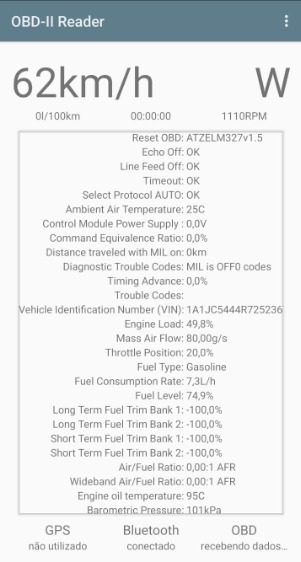
\includegraphics[scale=0.5]{figures/obd2.jpeg}
    
    \caption{Interface inicial do \textit{app} que se comunica com a porta OBD-II\textsuperscript{[12]}.}
    
    \label{fig:obd2_plataforma}
\end{figure}

    \subsection{Simulador de OBD-II}

    A ausência de um carro físico no início do projeto foi contornada por meio da utilização de um simulador de OBD. Esse dispositivo desempenhou um papel crucial como um substituto temporário do automóvel, permitindo que o trabalho continuasse normalmente. 
    
    Em vez de depender de um veículo real, a equipe conseguiu controlar e reproduzir dados e comportamentos típicos de um carro a partir do programa de controle do simulador\textsuperscript{[21]}.

    Além disso, o uso desse dispositivo proporcionou um ambiente controlado para a validação do \textit{software} em diferentes cenários, contribuindo para a eficiência e progresso do projeto enquanto não se podia realizar testes práticos.
    
    \subsection{Android Studio e Java} 
    A utilização da IDE Android Studio neste projeto de sistema de coleta de dados desempenha um papel central no desenvolvimento do aplicativo móvel já mencionado. 
    
    O Android Studio, sendo a principal ferramenta de desenvolvimento para aplicativos Android, oferece um ambiente integrado e robusto que simplifica a criação, os testes e a depuração do \textit{software}. 
    
    A plataforma fornece recursos avançados de \textit{design} de interface do usuário, facilitando a criação de aplicativos intuitivos e visualmente atraentes para os usuários finais. 
    
    A integração perfeita com o Android SDK (\textit{Software Development Kit}) permite o acesso às APIs e recursos específicos do sistema operacional Android, garantindo, através de interfaces do sistema operacional, o uso de \textit{hardwares} de propósito específico, como o que faz a comunicação Bluetooth. 
    
    Além disso, as ferramentas de emulação e depuração incorporadas no Android Studio simplificam o processo de teste em diferentes dispositivos, contribuindo para a criação de aplicativos estáveis e adaptáveis.

    Nenhuma tecnologia multiplataforma (React Native ou Flutter, por exemplo) ou específica de dispositivos iOS (Swift ou Objective C, por exemplo) foi escolhida, pois o intuito do projeto era ser compatível com os celulares dos membros do grupo e devido à familiaridade com a linguagem Java, usada para esse tipo de desenvolvimento.

    O aplicativo em si originalmente foi desenvolvido para a API de versão 22 do Android. Condição que foi alterada para comportar funcionalidades que foram adicionadas ao sistema operacional desde 2013. A versão atual de compilação (versão do SDK) é a 33.

    O desenvolvimento do aplicativo Android envolveu várias etapas, sendo o primeiro passo a modificação apropriada do arquivo \textit{build.gradle}. Este processo, no entanto, consumiu considerável tempo devido à falta de experiência dos membros do grupo. 
    
    Após a configuração inicial, a equipe se dedicou a identificar onde os parâmetros do OBD estavam disponíveis no código-fonte. Esta fase de investigação foi crucial para possibilitar o subsequente envio desses dados para a nuvem.

    No entanto, as dificuldades técnicas foram tão significativas que inicialmente não foi possível realizar o envio de dados para a nuvem. 
    
    Diante desse impasse, uma exceção teve que ser aberta no projeto, resultando na geração de arquivos \textit{.txt} locais no \textit{smartphone} em que o aplicativo estivesse rodando. 
    
    Essa solução permitiu que o trabalho de análise dos dados começasse, já que a produção de informações já estava funcional naquele momento.
    
    Posteriormente, a equipe conseguiu superar os obstáculos e implementou com sucesso o envio de dados para a nuvem, empregando a biblioteca Volley do Android. Essa abordagem proporcionou uma resolução eficaz para a integração com serviços de armazenamento na nuvem, consolidando a funcionalidade do \textit{app}. 

% \begin{figure}[hp]
%     \centering
    
%     
\includegraphics[scale=0.4]{figures/logo_android.png}
    
%     \caption{Logo do Android Studio.}
    
% \end{figure}
    
    \subsection{Banco de dados} 
    A integração do MySQL e do AWS RDS (Relational Database Service) em um projeto de sistema de compilação de dados de veículos é uma estratégia robusta para o gerenciamento eficiente e escalável dos dados do sistema. 
    
    O MySQL, um sistema de gerenciamento de banco de dados relacional de código aberto, proporciona uma estrutura confiável para armazenar e organizar informações como histórico de rotas e dados do OBD-II. 
     
     Ao escolher o AWS RDS como a plataforma de hospedagem para o MySQL, ganha-se os benefícios adicionais de escalabilidade automática, alta disponibilidade e segurança avançada oferecidos pela infraestrutura em nuvem da Amazon. A integração dessas tecnologias permite o acesso eficiente aos dados, consultas rápidas e uma gestão simplificada do banco de dados. 
     
     Além disso, o AWS RDS lida com tarefas operacionais, como \textit{backup} automático e manutenção. 
     
     Essa combinação proporciona uma base sólida para o armazenamento e recuperação de dados, promovendo a confiabilidade e eficácia do sistema.

     A estrutura definida para as tabelas do banco de dados foi:


    \begin{itemize}
         \item{\textbf{tcc-schema} (esquema do banco de dados onde se encontram as tabelas)}
         
        \begin{itemize}
             \item{\textbf{info:} Armazena as informações coletadas através da porta OBD} 
        
             \item{\textbf{acceleration:} Contém dados dos acelerômetros do celular do usuário} 
             
             \item{\textbf{location:} Guarda latitude e longitude obtidas por GPS pelo celular}   
        \end{itemize}  
    \end{itemize}

     A especificação exata das colunas de cada tabela pode ser encontrada no Apêndice 7.2.

    % \begin{figure}[hp]
    %     \centering
        
    %     
\includegraphics[scale=0.4]{figures/logo_Mysql.jpg}
        
    %     \caption{Logo do Mysql.}
        
    % \end{figure}

    Importante mencionar que o tamanho do banco de dados foi limitado a 20GiB, visando impedir que o serviço da AWS cobrasse qualquer valor monetário dos membros do grupo.
    
    O \textit{Free Tier} é um conjunto de limites de execução e armazenamento em nuvem definido para projetos-teste de contas novas na plataforma (com menos de 1 ano de existência\textsuperscript{[40]}). A forma de zerar os gastos com esse projeto é não exceder a fronteira dessas cortesias.

    
    \subsection{\textit{Python}} 

    A versão do Python usada para todos os arquivos \textit{.py} do projeto foi a 3.12.0.

    É importante mencionar que junto a cada módulo feito em Python neste projeto, as dependências necessárias para rodá-los foram escritas em arquivos \textit{requirements.txt}, como pode ser visto nos repositórios outrora mencionados.

%     As seguir um exemplo desse arquivo:

% \begin{python}
% ipykernel
% numpy
% pandas
% matplotlib
% folium
% geopy
% pyproj
% scipy
% plotly-express
% nbformat
% \end{python}

    Para poder-se executar os \textit{Jupyter Notebooks} desenvolvidos, é preciso desencadear os seguintes comandos em um terminal (em sistema operacional \textit{Linux}):

\begin{python}
python3 -m venv .venv
source .venv/bin/activate
python3 -m pip install requirements.txt
\end{python}
    

% \subsubsection{Folium}
     
%      A junção do Python e do Folium em um projeto de sistema de coleta de dados oferece uma poderosa combinação para a visualização interativa e geoespacial dos dados. 
     
%      O Folium é uma biblioteca que simplifica a criação de mapas interativos baseados na \textit{web}. Integrar o Folium ao projeto permite que os desenvolvedores gerem mapas dinâmicos que destacam informações específicas relacionadas ao rastreamento de veículos.

%     % Essa integração Python-Folium é particularmente útil para análises geoespaciais em sistemas de rastreamento de veículos, proporcionando uma representação geográfica e visualmente intuitiva dos dados de telemetria. 
    
%     % A flexibilidade do Python permite a personalização dos mapas e a incorporação de recursos adicionais conforme as necessidades específicas do projeto, contribuindo para uma interface de usuário mais informativa e envolvente.



% interface com usuario, banco de dados, conexão obd2

    % \subsubsection{Flask}

    % A seleção da biblioteca Flask para o projeto ocorreu devido à familiaridade com a linguagem Python, tornando o desenvolvimento mais acessível. Adicionalmente, a escolha se fundamentou na capacidade do Flask em facilitar a implementação eficiente de uma API, atendendo à necessidade do aplicativo de enviar e receber dados de maneira eficaz. O código python da API em Flask foi hospedado em um Lambda da AWS para facilitar o seu uso pelo APP posteriormente.


\section{Projeto e implementação}
% Esta seção descreverá as decisões feitas durante o trabalho.

% \subsection{Folium}
   

    \subsection{Análise de Dados - RideParser}\label{rideparser}

    A função da classe RideParser é analisar dados dos trajetos feitos pelos motoristas. 
    
    Alguns filtros são recebidos pelo construtor dessa classe, para personalizar a geração de gráficos. Esses parâmetros são usados para restringir o que vem do banco de dados a uma certa janela de tempo e ao usuário que solicita aquela informação.
    
    % Já o módulo 
    % ''os'' fornece funcionalidades relacionadas ao sistema operacional, permitindo que você interaja com o ambiente do sistema, como manipular diretórios, arquivos, obter informações sobre o sistema, manipular variáveis de ambiente, entre outras tarefas relacionadas ao sistema operacional.
    Dentro desse mesmo arquivo, algumas bibliotecas típicas de ciência de dados foram utilizadas para manipular os gráficos mencionados. Foram elas: pandas, matplotlib, numpy e scipy.
    
    A figura \ref{fig:rota_uah_driveset} mostra o video e o gráfico da aceleração de um carro. Os dados foram pegos de um repositório chamado UAH-Driveset\textsuperscript{[42]}, disponível na \textit{internet}.
    
    \begin{figure}[hp]
        \centering
        
        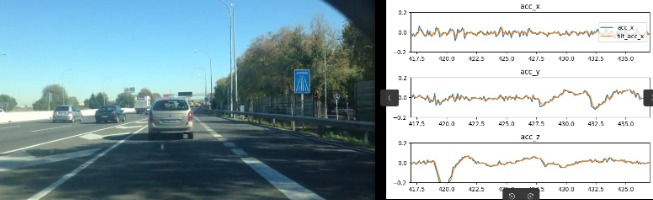
\includegraphics[scale=0.6]{figures/rota_uah_driveset.jpg}
        
        \caption{Rota de uma viagem de um dos integrantes do grupo.}
        \label{fig:rota_uah_driveset}
    \end{figure}

    \subsection{API Rest - Flask}
    A implementação da API centraliza-se em uma arquitetura Python utilizando a biblioteca Flask, proporcionando uma estrutura ágil e eficiente para a comunicação com a base de dados MySQL, hospedada em um serviço de RDS na AWS. A escolha da linguagem Python e do framework Flask foi motivada pela sua simplicidade e flexibilidade, permitindo a rápida construção dos \textit{endpoints} responsáveis pela interação entre o aplicativo e a base de dados.

    A lógica da API foi encapsulada em funções específicas, acionadas por meio de requisições POST. O corpo do JSON enviado nessas requisições determina a ação a ser executada, que pode ser uma entre seis operações distintas. Três destas operações referem-se a consultas (GET) e três a modificações (POST), cada uma vinculada a uma das três tabelas da base de dados.

    Para facilitar a utilização da API pelo \textit{app}, o código Python foi integrado ao ambiente \textit{serverless} da AWS Lambda. 
    
    Essa escolha estratégica permite que as funções sejam invocadas sob demanda, proporcionando uma resposta ágil às requisições do aplicativo Android, que, por sua vez, está sendo desenvolvido no ambiente Java do Android Studio. 
    
    A combinação dessas tecnologias promove uma arquitetura eficiente para gerenciar a comunicação entre o aplicativo e a infraestrutura de banco de dados na nuvem.

    \subsection{Folium}

% \begin{figure}[hp]
%     \centering
    
%     
\includegraphics[scale=0.1]{figures/python_folium.jpg}
    
%     \caption{Logos do Python e do Folium.}
% \end{figure}

 Para criar os mapas do aplicativo, foi utilizado o \textit{framework} Folium. Essa biblioteca é uma poderosa ferramenta para manipular e visualizar dados geoespaciais usando Python. 
    
    Com o Folium, é possível criar mapas interativos personalizados e incorporar dados neles de várias maneiras. Para manipular dados usando essa ferramenta, pode-se começar importando a biblioteca e criando um objeto \textit{Map}, que representa o mapa. 
    
    Em seguida, pode-se adicionar camadas, como marcadores, polígonos e \textit{popups}, para exibir dados de forma intuitiva no mapa. 
    
    % O Folium permite a integração de dados geoespaciais em diferentes formatos, como GeoJSON, tornando-o uma ferramenta flexível para análise e visualização de dados geoespaciais em Python. 
    
    A figura 
    \ref{fig:python_libs} mostra as bibliotecas utilizadas para desenvolver os mapas do projeto.
    
    \begin{figure}[hp]
        \centering
        
        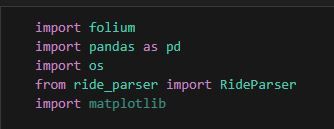
\includegraphics[scale=0.8]{figures/bibliotecas.jpg}
        
        \caption{Bibliotecas utilizadas para gerar o mapa da rota do usuário.}
        
        \label{fig:python_libs}
    \end{figure}
    
            % \begin{center}
            %  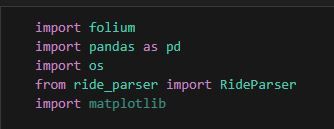
\includegraphics[scale=0.8]{figures/bibliotecas.jpg}
            %  
            %  \end{center}
            
    Para traçar uma trajetória no mapa usando a biblioteca Folium em Python, é necessária uma lista de pontos de latitude e longitude que representam a trajetória. 
    
    A partir dos pontos colhidos pelo GPS do celular, cria-se um mapa da trajetória descrita. A demonstração de uma trajetória recriada em um mapa usando Folium pode ser vista na figura \ref{fig:car_route_1}.
    
    \begin{figure}[hp]
        \centering
        
        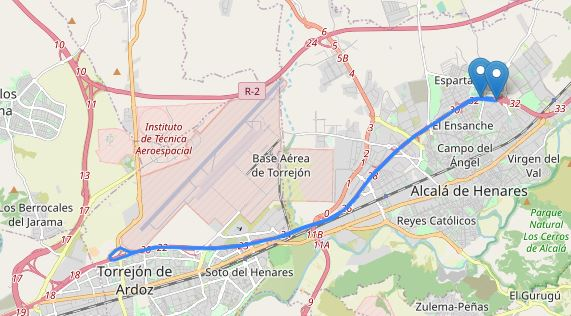
\includegraphics[scale=0.8]{figures/rota_1.jpg}
        
        \caption{Rota de uma das viagens fornecidas pelo \textit{UAH Driveset}.}
        
        \label{fig:car_route_1}
    \end{figure}
    
    O grupo procurou correlacionar eventos de anormalidade nos dados de aceleração do UAH Drivest observando o comportamento da curva dessa grandeza física no tempo e comparando com os eventos do vídeo que acompanhava cada uma das pastas disponibilizadas, mas nenhuma funcionalidade foi adicionada à análise dos dados devido a essa escolha.
    


    \subsection{Criação de relatório de direção em PDF}
    
    A geração de \textit{insights} visuais e análise métrica a partir dos dados armazenados na base MySQL é um componente essencial do projeto. 
    
    A decisão de fazer isso através da geração de um PDF para o motorista baseou-se na clareza e simplicidade desse formato de arquivo. 
    
    Essa escolha é respaldada também pela facilidade de implementação, disponibilizada pelas bibliotecas \textit{Matplotlib} e \textit{Reportlab}, que permitem a criação de PDFs formatados contendo os gráficos com as métricas geradas.
    
    Um segundo AWS Lambda desempenha papel central nesse processo, funcionando como uma ponte entre a base de dados e as ferramentas de visualização. 
    
    Ao ser acionado, o Lambda gerador de PDF realiza uma chamada ao outro Lambda, que extrai as informações relevantes da base de dados MySQL referentes ao usuário, para realizar a análise.

    Utilizando a biblioteca \textit{Matplotlib} em Python, a função Lambda então emprega métodos da classe RideParser, mencionada na seção \ref{rideparser}, para criar um relatório do motorista, com gráficos e métricas relevantes referentes a sua condução. Isso proporciona aos usuários uma compreensão mais aprofundada das métricas associadas às suas atividades.
    
    Para proporcionar aos usuários uma maneira acessível de interagir com esses \textit{insights}, um botão "gerar PDF" foi incorporado no aplicativo. Este botão aciona o segundo Lambda, que compila os gráficos e métricas gerados em um arquivo PDF. 
    
    A utilização da biblioteca \textit{smtplib} facilita o envio desse PDF diretamente para o usuário via \textit{email}. Essa solução integrada oferece uma experiência completa aos usuários, permitindo-lhes não apenas visualizar, mas também compartilhar os resultados de suas análises de maneira simples.    

    \subsection{Autenticação com \textit{Firebase}}

    A  escolha do \textit{Firebase} para a identificação única do usuário no sistema decorre da capacidade da plataforma em oferecer eficiência e segurança nesse processo, diminuindo-se a carga de responsabilidade do sistema em armazenar informações sensíveis de cada pessoa. 
    
    Essa decisão é fundamentada pela praticidade proporcionada pela integração do \textit{Firebase} com aplicativos \textit{Android} e páginas web\textsuperscript{[29]}, simplificando a implementação de autenticação e gestão de usuários, assegurando uma identificação singular e segura no âmbito do sistema em questão.

    \subsection{Dependências do Gradlle}

    Em um primeiro instante o \textit{app} android-obd-reader não rodava na IDE Android studio. 
    
    Para que fosse possível compilar o projeto, alterações no arquivo \textbf{gradle/wrapper/gradle-wrapper.properties} foram necessárias. 
    
    Atualizar as dependências do Gradle  é muitas vezes pré-condição para garantir que um aplicativo possa se beneficiar das correções de \textit{bugs}, melhorias de desempenho e novos recursos fornecidos pelas versões mais recentes das bibliotecas que estão sendo utilizadas. Este ponto na história do repositório mostra as alterações que foram necessárias: \url{https://github.com/APF2000/android-obd-reader-pires/commit/def70ed262b1fad28cc9e2b98a48af45cfac5695}.

    \subsection{Proteção dos dados}
    
    Na Lei Geral de Proteção de Dados (Lei n. 13.709/18-LGPD), parte-se da ideia de que todo dado pessoal tem importância e valor. 
    
    Por essa razão, este projeto levou em consideração o conceito amplo de dado pessoal, assim como estabelecido no Regulamento Europeu \textsuperscript{[30]} (\textit{GDPR-General Data Protection  Regulation}). 
    
    Quando se trata de um aplicativo projetado para analisar o perfil do motorista de carros, a LGPD impõe uma série de responsabilidades e requisitos ao desenvolvedor e operador do aplicativo. 
    
    É necessário obter o consentimento  do usuário antes de coletar e processar quaisquer dados pessoais relacionados ao seu perfil de condução.
    
    Além disso, a LGPD exige que medidas de segurança apropriadas sejam implementadas para proteger esses dados contra acessos não autorizados e vazamentos. Os usuários têm o direito de acessar, corrigir e excluir suas informações pessoais, e o aplicativo deve fornecer meios para que esses direitos sejam exercidos.

    Por simplicidade, este trabalho não cumpriu essas regras, mas o grupo tem ciência das vulnerabilidades e dos pontos de melhoria nesse aspecto.


% Using \texttt{biblatex} you can display a bibliography divided into sections, depending on citation type. 
% Let's cite! Einstein's journal paper \cite{einstein} and Dirac's book \cite{dirac} are physics-related items. 
% Next, \textit{The \LaTeX\ Companion} book \cite{latexcompanion}, Donald Knuth's website \cite{knuthwebsite}, \textit{The Comprehensive Tex Archive Network} (CTAN) \cite{ctan} are \LaTeX-related items; but the others, Donald Knuth's items, \cite{knuth-fa,knuth-acp} are dedicated to programming. 




\section{Testes e avaliação}
% descrever o plano de testes do sistema: testes de software, modulo, integração e validação
Alguns testes foram definidos para a ratificação das funcionalidades do sistema:

\begin{itemize}
    \item \textbf{Conferir conexão OBD-II:} 
    
    \begin{itemize}
        \item Conectar o dispositivo de leitura na entrada do carro
        \item Ligar a comunicação \textit{bluetooth} do celular
        \item Parear os dois dispositivos
        \item Digitar a senha 1234, padrão dos dispositivos de leitura OBD
        \item Ligar a coleta de dados através do aplicativo
        \item A tela deve sinalizar que o protocolo está sendo feito da forma correta
    \end{itemize}
    
    \item \textbf{Teste de continuidade de transferência de dados:} 
    \begin{itemize}
        \item Fazer conexão com o OBD conforme descrito no teste anterior
        \item Andar com o carro por alguns minutos com a tela do celular desbloqueada (de preferência mudar o \textit{timeout} da tela nas configurações do celular)
        \item Atestar que nenhum dado foi perdido por falta de conexão (pode ser visto por descontinuidade dos gráficos)
    \end{itemize}
    
    \item \textbf{Equivalência de envio e recepção de dados:}
    \begin{itemize}
        \item Comparar o \textit{log} de envio de dados do aplicativo de interface com a porta OBD-II com o \textit{log} de salvamento do banco de dados hospedado na nuvem
        \item A quantidade de dados, os \textit{timestamps} deles e seus conteúdos devem ser idênticos
    \end{itemize}
    
    \item \textbf{Testes de segurança:} 
    \begin{itemize}
        \item Ratificar que não é possível ter acesso aos dados de um certo usuário sem ter as informações de \textit{login}
        \item Verificar o certificado SSL do remetente e só aceitar a mensagem se a informação condisser com as credenciais armazenadas daquele usuário
    \end{itemize}
    
    \item \textbf{Geração de dados \textit{outliers}:}
    \begin{itemize}
        \item Verificar se o sistema descarta corretamente as informações que fogem totalmente do padrão esperado ou se consegue pelo menos esconder isso do usuário
        \item Os PDFs gerados com o sistema devem sofrer um processo de análise de plausibilidade, o que deve averiguar que a análise automática está sendo feita corretamente
    \end{itemize}
    
\end{itemize}


\subsection{Fluxo de uso do sistema}

    \begin{itemize}
    \item \textbf{Autenticação com o Google:}
    O aplicativo no celular deve ser iniciado para realizar a autenticação com as credenciais do Google, assegurando uma identificação segura do usuário.

    \item \textbf{Conexão com o OBD:}
    A conexão entre o celular e o OBD deve ser estabelecida, garantindo que o leitor esteja corretamente emparelhado para iniciar a comunicação.

    \item \textbf{Início da Coleta de Dados:}
    A coleta de dados deve ser ativada por meio do aplicativo.

    \item \textbf{Condução do Veículo:}
    O veículo deve ser conduzido normalmente, permitindo que o aplicativo faça a coleta de dados em tempo real.

    \item \textbf{Posicionamento Fixo do Celular:}
    O celular deve ser fixado em uma posição estável dentro do veículo usando um suporte apropriado. Isso garantirá que os dados de aceleração sejam confiáveis, o que evitará qualquer tipo de interferência na análise posterior da direção.
\end{itemize}


\subsection{Carros utilizados para teste}

    A escolha dos carros onde o leitor de OBD seria conectado foi feita a partir dos veículos de familiares.

    Os modelos em que o sistema foi testado, foram em maioria para analisar quais parâmetros de OBD haviam sido implementados em todos eles.

    Os carros usados foram:

    \begin{itemize}
        \item Hyundai Ix35 - 2012
        \item Mercedes C200 CGI - 2014
        \item Ford Xsport - 2008
    \end{itemize}

    
    O modelo Ix35 foi a principal fonte de dados do projeto, pois praticamente todos os testes feitos para a nova base de dados foram feitos com ele.

    \subsection{Aparelhos \textit{smartphone}}

    O aplicativo foi rodado em dois modelos diferentes de celular:
    \begin{itemize}
        \item Samsung Galaxy A71
        \item Samsung Galaxy S9
        \item Samsung Galaxy S22
        \item Motorola Moto G
    \end{itemize}

\subsection{Definição de dados relevantes para o perfilamento}

    Os parâmetros identificados em comum em todos os carros testados foram: \textit{AIR-FUEL-RATIO, AIR-INTAKE-TEMP, AMBIENT-AIR-TEMP, BAROMETRIC-PRESSURE, CONTROL-MODULE-VOLTAGE, DISTANCE-TRAVELED-MIL-ON, DTC-NUMBER, ENGINE-COOLANT-TEMP, ENGINE-LOAD, ENGINE-OIL-TEMP, ENGINE-RPM, ENGINE-RUNTIME, EQUIV-RATIO, Echo Off, FUEL-CONSUMPTION-RATE, FUEL-LEVEL, FUEL-PRESSURE, FUEL-RAIL-PRESSURE, FUEL-TYPE, INTAKE-MANIFOLD-PRESSURE, Line Feed Off, Long Term Fuel Trim Bank 1, Long Term Fuel Trim Bank 2, MAF, Reset OBD, SPEED, Select Protocol AUTO, Short Term Fuel Trim Bank 1, Short Term Fuel Trim Bank 2, THROTTLE-POS, TIMING-ADVANCE, TROUBLE-CODES, Timeout, VIN, WIDEBAND-AIR-FUEL-RATIO}.

    No entanto, muitas dentre essas informações ou apresentavam o valor \textit{NODATA}, que significa que estavam sendo amostrados pelo OBD, mas não continham dados válidos, ou apresentavam dados constantes, os quais independem da direção do motorista.

    Os \textbf{parâmetros descartados} foram \textit{CONTROL-MODULE-VOLTAGE, DISTANCE-TRAVELED-MIL-ON, DTC-NUMBER, Echo Off, ENGINE-OIL-TEMP, FUEL-CONSUMPTION-RATE, FUEL-LEVEL, FUEL-PRESSURE, FUEL-RAIL-PRESSURE, FUEL-TYPE, Line Feed Off, Long Term Fuel Trim Bank 2, MAF, Reset OBD, Select Protocol AUTO, Short Term Fuel Trim Bank 2, Timeout, TROUBLE-CODES, VIN, WIDEBAND-AIR-FUEL-RATIO}.
    
    Os \textbf{parâmetros considerados} para uso foram \textit{AIR-FUEL-RATIO, AIR-INTAKE-TEMP, AMBIENT-AIR-TEMP, BAROMETRIC-PRESSURE, ENGINE-COOLANT-TEMP, ENGINE-LOAD, ENGINE-RPM, ENGINE-RUNTIME, EQUIV-RATIO, INTAKE-MANIFOLD-PRESSURE, Long Term Fuel Trim Bank 1, Short Term Fuel Trim Bank 1, SPEED, THROTTLE-POS, TIMING-ADVANCE}.
    
    Entre os dados candidatos para serem usados no projeto, apenas os que foram \textbf{citados em artigos científicos} como determinantes para o acontecimento de acidentes e a deterioração do carro foram de fato levados em consideração: \textit{ENGINE-RPM}\textsuperscript{[28]}, \textit{SPEED}\textsuperscript{[32]}

            %     \item CONTROL-MODULE-VOLTAGE
            % \item DISTANCE-TRAVELED-MIL-ON
            % \item DTC-NUMBER
            % \item Echo Off
            % \item ENGINE-OIL-TEMP
            % \item FUEL-CONSUMPTION-RATE
            % \item FUEL-LEVEL
            % \item FUEL-PRESSURE
            % \item FUEL-RAIL-PRESSURE
            % \item FUEL-TYPE
            % \item Line Feed Off
            % \item Long Term Fuel Trim Bank 2
            % \item MAF
            % \item Reset OBD
            % \item Select Protocol AUTO
            % \item Short Term Fuel Trim Bank 2
            % \item Timeout
            % \item TROUBLE-CODES
            % \item VIN
            % \item WIDEBAND-AIR-FUEL-RATIO

            % \item AIR-FUEL-RATIO
            % \item AIR-INTAKE-TEMP
            % \item AMBIENT-AIR-TEMP
            % \item BAROMETRIC-PRESSURE
            % \item ENGINE-COOLANT-TEMP
            % \item ENGINE-LOAD
            % \item ENGINE-RPM
            % \item ENGINE-RUNTIME
            % \item EQUIV-RATIO
            % \item INTAKE-MANIFOLD-PRESSURE
            % \item Long Term Fuel Trim Bank 1
            % \item Short Term Fuel Trim Bank 1
            % \item SPEED
            % \item THROTTLE-POS
            % \item TIMING-ADVANCE


    % \begin{itemize}
    %     \item AIR-FUEL-RATIO
    %     \item AIR-INTAKE-TEMP
    %     \item AMBIENT-AIR-TEMP
    %     \item BAROMETRIC-PRESSURE
    %     \item CONTROL-MODULE-VOLTAGE
    %     \item DISTANCE-TRAVELED-MIL-ON
    %     \item DTC-NUMBER
    %     \item ENGINE-COOLANT-TEMP
    %     \item ENGINE-LOAD
    %     \item ENGINE-OIL-TEMP
    %     \item ENGINE-RPM
    %     \item ENGINE-RUNTIME
    %     \item EQUIV-RATIO
    %     \item Echo Off
    %     \item FUEL-CONSUMPTION-RATE
    %     \item FUEL-LEVEL
    %     \item FUEL-PRESSURE
    %     \item FUEL-RAIL-PRESSURE
    %     \item FUEL-TYPE
    %     \item INTAKE-MANIFOLD-PRESSURE
    %     \item Line Feed Off
    %     \item Long Term Fuel Trim Bank 1
    %     \item Long Term Fuel Trim Bank 2
    %     \item MAF
    %     \item Reset OBD
    %     \item SPEED
    %     \item Select Protocol AUTO
    %     \item Short Term Fuel Trim Bank 1
    %     \item Short Term Fuel Trim Bank 2
    %     \item THROTTLE-POS
    %     \item TIMING-ADVANCE
    %     \item TROUBLE-CODES
    %     \item Timeout
    %     \item VIN
    %     \item WIDEBAND-AIR-FUEL-RATIO
    % \end{itemize}
\chapter{Considerações finais}

Este capítulo descreve as observações posteriores à conclusão do projeto.

\section{Conclusões do projeto de formatura}
% "foi bom, tivemos que mudar isso e isso e isso"
Esta seção será modificada quando o projeto tiver sido implementado.

\section{Contribuições}
% qual foi a contrib da equipe
Esta seção será modificada quando o projeto tiver sido implementado.

\section{Perspectivas de continuidade}
% o que pode ser feito depois do tcc?
Embora o projeto ainda não tenha acabado, já é possível vislumbrar o que pode ser feito com o sistema que será desenvolvido.

A ideia principal dos itens listados a seguir é a de fazer uso da plataforma de dados como ferramenta principal de fornecimento de dados:

\begin{itemize}
    \item \textbf{Classificador de perfil de direção para seguros de carro personalizados:} valores mais altos para motoristas mais violentos.
    
    \item \textbf{Prova de direção conduzida por Inteligência Artificial:} possível supressão da prova do Detran, avaliando o condutor ao longo das aulas práticas.
    
    \item \textbf{Ranqueador de segurança de carros autônomos:} avaliação dos carros do futuro para determinar qual dirige com mais segurança.
    
    \item \textbf{Revisão remota / diagnóstico automático de carro:} relatar problemas antes que aconteçam, sem a necessidade de um mecânico para examinar diretamente o veículo.
    
    \item \textbf{Classificação de motoristas de aplicativo:} avaliação ponderada pela forma de dirigir
\end{itemize}
% \chapter{Apêndices}

Como juntar todas as subpartes do projeto é uma outra tarefaimportante de engenharia.

A seguir é descrito como isso pode ser feito.

\section{Compra da placa ATMEGA}
\section{Compra da placa ATMEGA}
\section{Compra da placa ATMEGA}
\section{Compra da placa ATMEGA}
\section{Compra da placa ATMEGA}
% \chapter{Anexos}

Este capítulo tem como objetivo 


\section{eeeeeeeeeeeeeeeeee}\label{Sub:equa}

Usaremos as bibliotecas de cada sensor e motor a ser usado, para facilitar a integração
Não há necessidade de sistema de arquivos, já que os dados são tratados ativamente
Usaremos os drivers de interface com o GPIO fornecidos pelo SO
A depuração será feita em cada camada de maneiras diferentes: 
Simulação → aplicação 
QEMU → SO 
LEDs → hardware 

\chapter{Referências}

\urlstyle{same} % mantém fonte das letras que compõem url

[1] \textbf{US20130052614A1 - Driver Performance Metric}. Google Patents, 2012. Disponível em <\url{patents.google.com/patent/US20130052614}>. Acesso em 30 de jan. de 2023.

[2] \textbf{CAMPO GRANDE}, Paulo. "Novas Tecnologias: Carros Atuais Têm Até 100 Sensores a Bordo." Revista Quatro Rodas, Brasil, 12 de jun. de 2018. Disponível em <\url{quatrorodas.abril.com.br/noticias/novas-tecnologias-carros-atuais-tem-ate-100-sensores-a-bordo/}>. Acesso em 20 de fev. de 2023.

% 17 de mar de 
[3] WIKIMEDIA Foundation. \textbf{OBD-II PIDs}. Wikipedia, 2023. Disponível em <\url{en.wikipedia.org/wiki/OBD-II_PIDs}>. Acesso em 20 de mar. de 2023

% 9 de set. de 
[4] FINCO, Nina. \textbf{OBD}: o Que é e Para Que Serve o Protocolo OBD2?. Cobli Blog, 2021. Disponível em <\url{www.cobli.co/blog/o-que-e-protocolo-obd2/}>. Acesso em 20 de mar. de 2023.

% 25 de nov. de
[5] BARRETO, Victor. \textbf{What Is OBDII?} History of on-Board Diagnostics. Geotab, 2020 Disponível em <\url{www.geotab.com/blog/obd-ii/}>. Acesso em 20 de mar. de 2023.

[6] SBT News. \textbf{No Brasil, cerca de 32 pessoas morrem por dia em acidentes de trânsito}. SBT, Brasil, 22 de jan. de 2022. Disponível em <\url{www.sbtnews.com.br/noticia/brasil/194388-no-brasil--cerca-de-32-pessoas-morrem-por-dia-em-acidentes-de-transito#:~:text=Em 2021, foram 11.647 mortes,incidentes por hora no Brasil.}>. Acesso em 23 de abr. de 2023.

[7] \textbf{ACIDENTES De Trânsito São a Maior Causa De Morte De Pessoas De 5 a 29 Anos}. ONU News. Nações Unidas, 21 de nov. de 2021. Disponível em <\url{news.un.org/pt/story/2021/11/1771092}>. Acesso em 18 de abr. de 2023.

[8] \textbf{TOTAL Confirmed COVID-19 Deaths}. Our World in Data, 2023. Disponível em <\url{ourworldindata.org/grapher/covid-deaths-income}>
. Acesso em 18 de abr. de 2023.

[9] \textbf{Em Quanto Tempo Os Carros Autônomos Serão o Novo 'Padrão'?}. Jaguar Brasil. Disponível em <\url{www.jaguarbrasil.com.br/news/em-quanto-tempo-os-carros-autonomos-serao-o-novo-padrao.html#:~:text=A indústria de pesquisa IHS,pode demorar um pouco mais}>. Acesso em 23 de abr. de 2023.


[10] \textbf{PREÇO sob demanda do Amazon EC2}. Amazon. Disponível em <\url{aws.amazon.com/pt/ec2/pricing/on-demand/}>. Acesso em 23 de abr. de 2023.


[11] \textbf{CALCULADORA de preço}. Microsoft Azure. Disponível em <\url{azure.microsoft.com/de-de/pricing/calculator/}>. Acesso em 23 de abr. de 2023.

[12] \textbf{PIRES}. "Android OBD-II Reader Application That Uses Pure OBD-II PID's Java API." GitHub. Disponível em <\url{github.com/pires/android-obd-reader}>. Acesso em 23 de abr. de 2023.

[13] \textbf{PAGE}, Vanessa. "Waze: The Pros and Cons." Investopedia, 12 de jan de 2023. Disponível em <\url{www.investopedia.com/articles/investing/060415/pros-cons-waze.asp#:~:text=Waze uses data from app,that could slow down drivers}>. Acesso em 23 de abr. de 2023.


[14] \textbf{Scanner Automotivo Conector Obd2 Elm327 Bluetooth}. Mercado Livre, <\url{produto.mercadolivre.com.br/MLB-2147325216-scanner-automotivo-conector-obd2-elm327-bluetooth-_JM#position=1&search_layout=grid&type=pad&tracking_id=509523dc-c530-481c-954c-0ecbe9c6a94c&is_advertising=true&ad_domain=VQCATCORE_LST&ad_position=1&ad_click_id=ODlhMjFlMzctNjQ5Ni00MTg1LWIzYWYtZjk3Y2U5MjlmNjNm}>. Acesso em 23 de abr. de 2023.

[15] \textbf{SAIPRASERT}, Chalermpol. et al. "Driver Behaviour Profiling Using Smartphone Sensory Data in a V2I Environment". 2014 International Conference on Connected Vehicles and Expo (ICCVE), 2014. Disponível em <\url{https://ieeexplore.ieee.org/abstract/document/7297609}>. Acesso em 24 de abr. de 2023.

[16] \textbf{Imagem MySql e AWS RDS}. Disponível em <\url{https://medium.com/99dotco/our-mysql-rds-upgrade-journey-cutting-down-downtime-by-11200-and-lessons-learned-1fa828e6009c}>. Acesso em 20 de nov. de 2023.

[17] \textbf{Imagem Python e Folium}. Disponível em <\url{https://www.google.com/url?sa=i&url=https%3A%2F%2Fm.youtube.com%2Fwatch%3Fv%3D4RnU5qKTfYY&psig=AOvVaw05zKbpT4lYD0v7v8M3hIZe&ust=1700594334592000&source=images&cd=vfe&opi=89978449&ved=0CA8QjRxqFwoTCMCfq-Kl04IDFQAAAAAdAAAAABAD}>. Acesso em 20 de nov. de 2023.

[18] \textbf{Simulador Carla.} Disponível em <\url{https://carla.org/}>. Acesso em 11 de dez. de 2023.

[19] \textbf{Site Rota2030.} Disponível em <\url{https://www.rota2030.com.br/}>.  Acesso em 11 de dez. de 2023.

[20] \textbf{Dosovitskiy, A., Ros, G., Codevilla, F., Lopez, A., Koltun, V. (2017, October)}. "CARLA: An open urban driving simulator." In Conference on robot learning (pp. 1-16). PMLR.

[21] \textbf{Simulador OBD-II} Disponível em <\url{https://freematics.com/store/index.php?route=product/product&product_id=71}>. Acesso em 11 de dez. de 2023.


[22] \textbf{Ferreira Júnior, Jair da Silva}.
"Análise de Perfil de Motoristas : Uma Investigação com Diferentes Sensores e Técnicas de
Aprendizado de Máquina / Jair da Silva Ferreira Júnior. — 2018"
101 f. : il. color.

[23] \textbf{Shibata, Danilo Jun; Soares, Leandro Donizetti}. "Análise de Direção de motoristas Utilizando o Protocolo OBD2 e sensores Embarcados."

[24] \textbf{Bethge, Johanna, et al}."Model Predictive Control with Gaussian-Process-Supported Dynamical Constraints for Autonomous Vehicles." arXiv preprint arXiv:2303.04725 (2023).

[25] \textbf{Ferreira J Júnior, Carvalho E, Ferreira BV, de Souza C, Suhara Y, et al. (2017)}. "Driver behavior profiling: An investigation with different smartphone sensors and machine learning." PLOS ONE 12(4): e0174959.

[26] \textbf{Júnior, J. Ferreira, and Gustavo Pessin}. "Análise de perfil de motoristas: Detecção de eventos por meio de smartphones e aprendizado de máquina." Anais do WOCCES 2016 Workshop de Comunicação em Sistemas Embarcados Críticos. 2016.

[27] \textbf{Documentação dos acelerômetros para desenvolvimento Android.} Disponível em <\url{https://developer.android.com/develop/sensors-and-location/sensors/sensors_overview}>. Acesso em 11 de dez. de 2023.

[28] \textbf{Seifi, Mohammad Reza, et al.} "Experimental investigation of a diesel engine power, torque and noise emission using water–diesel emulsions." Fuel 166 (2016): 392-399.

[29] \textbf{Documentação do OneTapSignIn do Firebase.} Disponível em <\url{https://firebase.google.com/docs/auth/android/google-signin?hl=pt-br}>. Acesso em 11 de dez. de 2023.

[30] \textbf{Plataforma de seguro de vida com preço dinâmico.} Disponível em <\url{https://www.azos.com.br}>. Acesso em 11 de dez. de 2023.

[31] \textbf{de TEFFÉ, Chiara Spadaccini, and Mario Viola. } "Tratamento de dados pessoais na LGPD: estudo sobre as bases legais." \textbf{civilistica.com}, v. 9, n. 1, p. 1-38, 9 maio 2020. Acesso em 11 de dez. de 2023.

[32] \textbf{Garber, Nicholas J.; Gadirau, Ravi.} "Speed Variance and Its Influence on Accidents." AAA Foundation for Traffic Safety, 1730 M Street, N.W., Suite 401, Washington, DC 20036.



%%%% Estilo de citação ABNT e arquivo de bibitens (mybibliography.bib)
% \bibliographystyle{abnt-alf}
% \bibliography{mybibliography}
% \printbibliography


\chapter{Referências}

[1] “US20130052614A1 - Driver Performance Metric.” Google Patents, Google, disponível em <patents.google.com/patent/US20130052614>. Acesso em 30 de janeiro de 2022

[2] Paulo Campo Grande. “Novas Tecnologias: Carros Atuais Têm Até 100 Sensores a Bordo.” Quatro Rodas, 12 de junho de 2018, disponível em <quatrorodas.abril.com.br/noticias/novas-tecnologias-carros-atuais-tem-ate-100-sensores-a-bordo/>. Acesso em 20 de fevereiro de 2022

[3] “OBD-II PIDs.” Wikipedia, Wikimedia Foundation, 17 Mar. 2022, disponível em <en.wikipedia.org/wiki/OBD-II_PIDs>. Acesso em 20 de março de 2022

[4] Sobre o autor Nina Finco Formada em jornalismo pela UMESP-SP e especialista em mídia. “OBD: o Que é e Para Que Serve o Protocolo OBD2?” Blog Da Cobli, 9 Sept. 2021, disponível em <www.cobli.co/blog/o-que-e-protocolo-obd2/>. Acesso em 20 de março de 2022

[5] “What Is OBDII? History of on-Board Diagnostics.” Geotab, disponível em <www.geotab.com/blog/obd-ii/>. Acessado em 20 de março de 2022

[6] https://www.sbtnews.com.br/noticia/brasil/194388-no-brasil--cerca-de-32-pessoas-morrem-por-dia-em-acidentes-de-transito#:~:text=Em%202021%2C%20foram%2011.647%20mortes,incidentes%20por%20hora%20no%20Brasil.

[7] https://news.un.org/pt/story/2021/11/1771092

[8] https://ourworldindata.org/grapher/covid-deaths-income, consultado em 18 de abril de 2022

[9] https://www.jaguarbrasil.com.br/news/em-quanto-tempo-os-carros-autonomos-serao-o-novo-padrao.html#:~:text=A%20ind%C3%BAstria%20de%20pesquisa%20IHS,pode%20demorar%20um%20pouco%20mais.



\newpage
% \referencias
% \bibliography{bib/bib.bib}


% \printbibliography[
%     heading=bibintoc,
%     title={Referências}
% ] %Prints the entire bibliography with the title "Whole bibliography"

% \apendice
% \include{appendices}




\end{document}